\chapter{Reconstruction}
\label{annex:detectors-sc-physics-software-reconstruction}

The raw data from the near and far detectors provide highly detailed views of neutrino
interactions and background events, which must be reduced and interpreted in order to
extract the physics measurements.  Cosmic rays must be identified and rejected, tracks and
showers selected, particle identities assigned to the reconstructed objects, and event-level
interpretations formed.  While the performance of the reconstruction in both the Near Detector
and the Far Detector have direct impacts on the physics sensitivity of the experiment, effects
resulting from the detector designs and the angular and momentum acceptance differences of the
near and far detectors are ingredients in the systematic uncertainty estimations that also
affect the sensitivity of the experiment.  If a particular class of events has a different
reconstruction efficiency or energy resolution in the near and the far detectors, then modeling of the fraction of events
in this class may become important, and cross sections and nuclear modeling systematic uncertainties
can enter in this way.  The fact that the near detector is smaller than the far detector and accepts a larger
angular range of particles from the beam will introduce some of the systematic uncertainties even if the
technologies are the same. 

\section{Near Detector Reconstruction}
\label{annex:detectors-sc-physics-software-reconstruction-nd}

The Near Detector full reconstruction has not been developed yet, though a parameterized event
reconstruction of the ND FastMC (described in section \ref{annex:detectors-sc-physics-software-simulation-nd})
has been developed and used for physics sensitivity studies.  In the ND FastMC, particles are ``reconstructed''
by applying the smearing function shown in Tab.~\ref{tab:ndfastmc_par}.  The parameters of the smearing
function are guided by NOMAD detector performance~\cite{Anfreville:2001zi}.  Fig.~\ref{fig:ndfastmc_mures} shows
the momentum resolution in $\nu_\mu$-CC obtained from the ND FastMC simulation and reconstruction framework with DUNE ND flux.

\begin{cdrfigure}[Near Detector muon momentum resolution]{ndfastmc_mures}
{The distribution of fractional differences of measured muon momenta from their true values 
for smeared muon tracks in $\nu_\mu$-CC events using the Near Detector's FastMC parameterization.  The distribution
of $\delta p_\mu/p_\mu$ is shown with a blue histogram and a fit to a single Gaussian is shown with a red curve.  The
Gaussian fit gives an average resolution of 3.3\%.
}
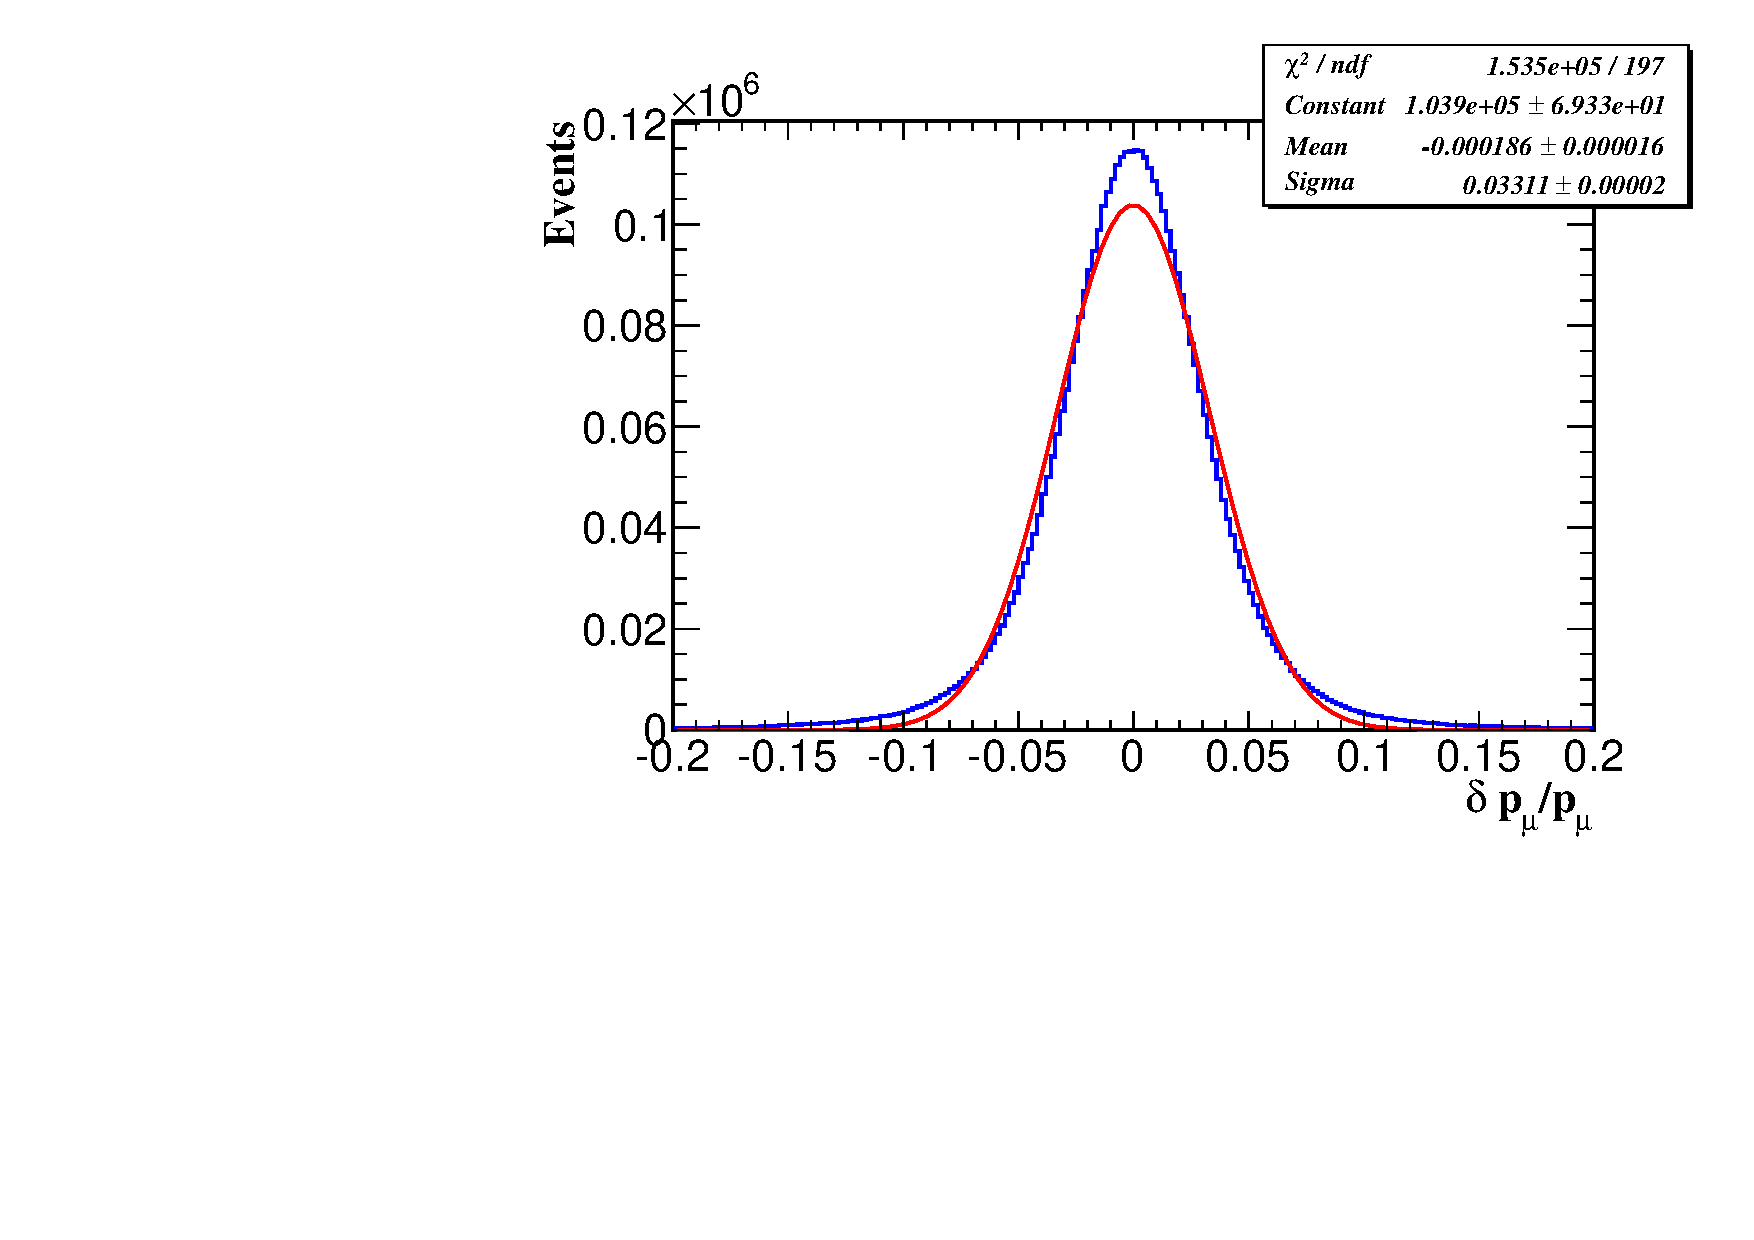
\includegraphics[width=0.8\textwidth]{ndfastmc_mures.pdf}
\end{cdrfigure}

Along with the GEANT4 full simulation of the near detector, additional effort will be directed
towards reconstruction with the aim of guiding the optmization of the near detector design by 2018.

\section{Far Detector Reconstruction}
\label{annex:detectors-sc-physics-software-reconstruction-fd}

The reconstruction of particle interactions in Liquid Argon TPC
detectors is an active area of research and development.
A series of sophisticated reconstruction algorithms are required to
address a broad range of complex event topologies, and to perform
precise physics measurements that fully exploit the spatial and 
calorimetric precision offered by Liquid Argon technology.
Although the field is not yet mature, there has been considerable
progress in recent years, including the first fully automated
pattern recognition algorithms. 

A fully automated event reconstruction is being developed for the
DUNE Far Detector, and major pieces are in place and functioning.
The single-phase reconstruction algorithms are developed in LArSoft~\cite{Church:2013hea},
which is based on the {\it art} framework~\cite{Green:2012gv}.  The dual-phase reconstruction
algorithms are incorporated in Qscan~\cite{lussi:thesis}.
The block diagram in Figure~\ref{fig:fdrecoblockdiag}
illustrates the components of the far detector reconstruction chain.  The main steps and
their ordering is similar between the single-phase and the dual-phase software designs
and may evolve as experience is gained. 
The first stage involves the processing of the noisy ADC wire signals,
and creation of 2D `hits'. A series of pattern recognition algorithms
are then used to group the hits into 2D and 3D clusters representing 
individual particle tracks and showers. A set of high-level tools
then reconstructs the vertex and 3D trajectory of each particle,
provides particle identification, and reconstructs the four-momentum.
While each step of the reconstruction chain has been implemented,
the algorithms have not yet been fully optimized.
The following sections describe the current status of each task.

\begin{cdrfigure}[Far detector reconstruction block diagram]{fdrecoblockdiag}
{Block diagram showing the components of the far detector reconstruction chain}
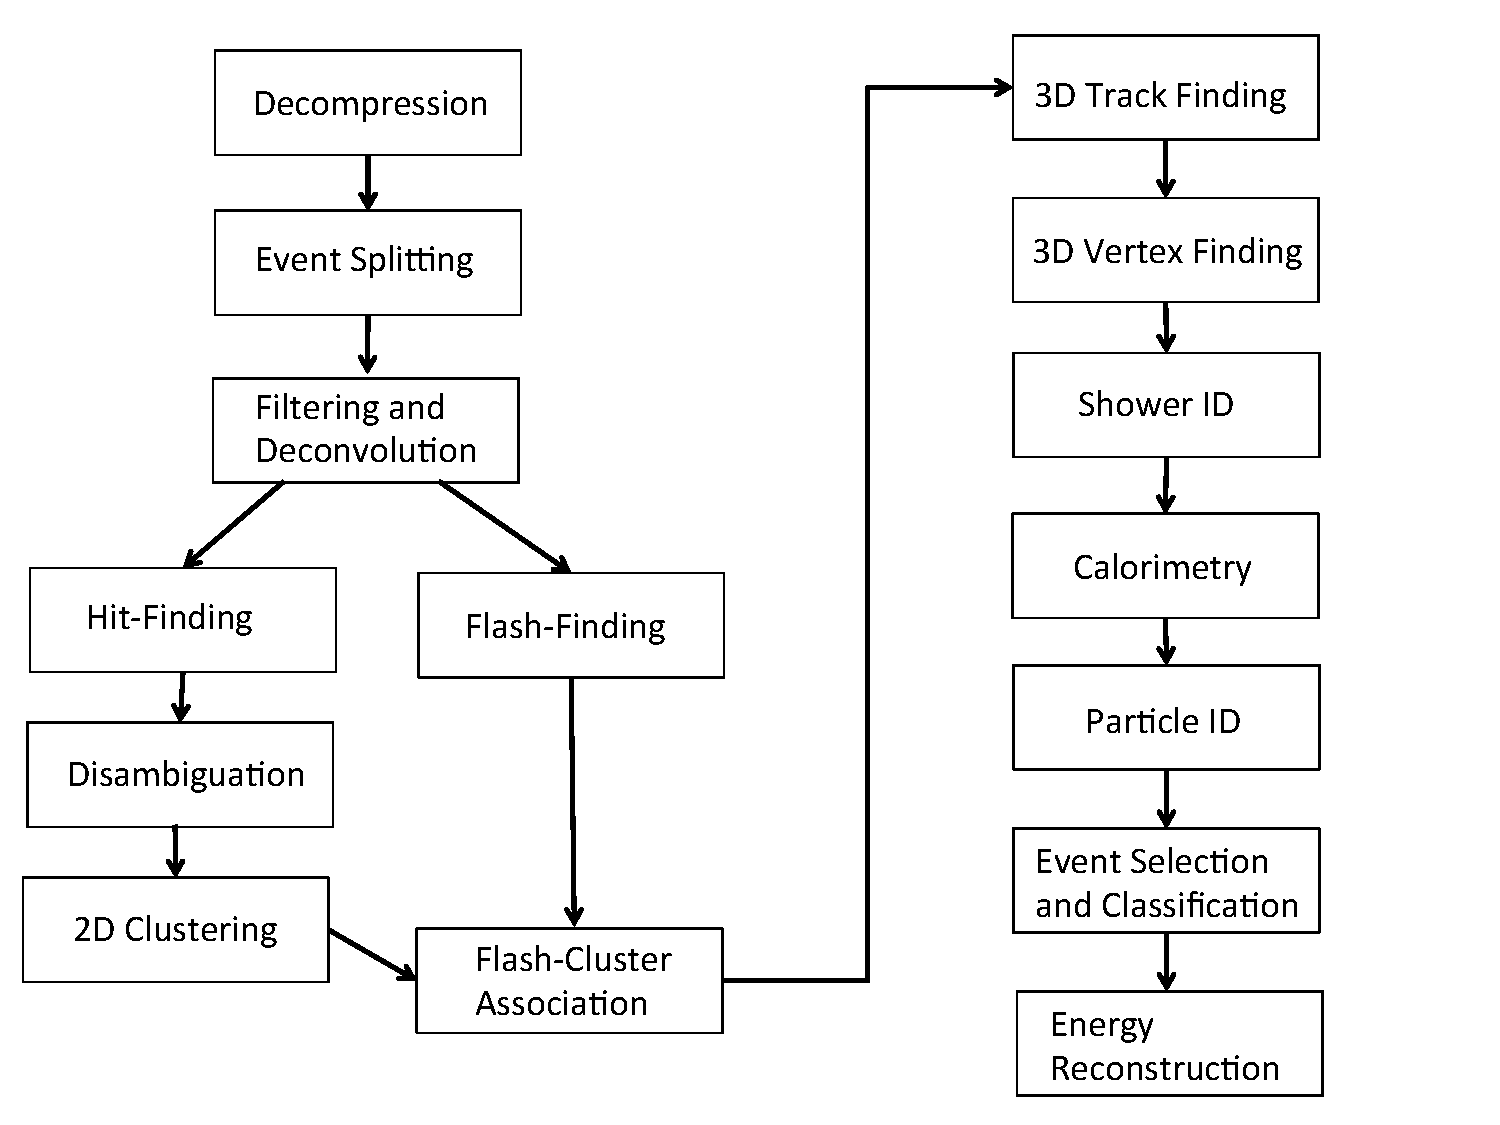
\includegraphics[width=\textwidth]{fdrecoflowchart_annex.pdf}
\end{cdrfigure}

\subsection{Signal Processing and Filtering}
\label{annex:reconstruction-signal-proc}

A series of signal processing algorithms has been developed to
perform noise reduction and baseline subtraction on the digital
waveforms read out by Liquid Argon TPC detectors. 

The TPC data are first uncompressed and put into local storage, one channel at a time.  
In the case that the DAQ writes data records to persistent
storage the correspond to inconveniently long time periods, the data may be split
into smaller events at the readin stage.  At this stage, if an interaction is found
to have taken place near the edge of the time corresponding to one record from the DAQ,
the next DAQ record may be appended to make an offline event that corresponds to
what is required to analyze the interaction of interest.

\subsubsection{Single-Phase Signal Processing and Filtering}

The single-phase detector's bipolar induction-plane pulses must be deconvolved,
since the negative portions of pulses may cancel positive portions of pulses on the channel
that are nearby in time, even if the charge in those pulses is deposited on distant segments
of the wire.  Deconvoluting the bipolar signals produces unipolar pulses that can be fit in the
same way as for the collection plane's unipolar signals.  
The electronics response as well as the detector response is included in the
deconvolution, and so deconvolution also of the collection-plane signals is also performed to improve
the resolution.   Since the deconvolution is performed by multiplying the Fourier transform of the
input raw data by a deconvolution kernel, it is convenient to apply a frequency-dependent noise filter
at this stage before transforming the data back into the time domain.
A computational speedup is achieved by packing data in
blocks that exceed thresholds plus nearby neighbors in time so that
the FFT only needs to see a fraction of the total ADC samples
collected in each event.
The detector response functions used to construct the deconvolution kernels are currently
based on \textit{a priori} predictions, but these will be tuned and
validated using data from the 35-ton prototype and the~\cernsingleproto{} at CERN.
It may be necessary to filter unipolar signal components on the induction-plane
wires and handle these signals separately, in the case of partial
non-transparency of the induction planes, which might be unavoidable
near the wrapping boundaries.  

\subsubsection{Dual-Phase Signal Processing and Filtering}

Qscan~\cite{lussi:thesis} also provides a set of methods for signal processing. 
The raw waveforms are first processed: this involves noise reduction as well as the subtraction of the baseline.
Hits, defined as signals that are discriminated from the noise, are identified and reconstructed.
In order to suppress noise without affecting the signal component too much, hence improving the signal to noise ratio, 
two different algorithms are used: the Fast Fourier Transform (FFT) filter, and the coherent noise subtraction algorithm.
A smooth cut-off, implemented with a Fermi potential, efficiently suppresses the noise without introducing artifacts in the
time domain.
The coherent noise filter is implemented to remove identical noise patterns that are seen on larger sets of readout channels. 
Unlike in the case of the FFT filter, which directly suppresses the frequencies of single 
channels and thus reducing the signal bandwidth, the coherent noise filter ideally subtracts only the noise while keeping the signals unchanged.
After suppressing the noise, the (constant) pedestal of each waveform has to be computed and subtracted from each sample.

\subsection{TPC Hit Finding}
\label{annex:reconstruction-single-phase-hit-find}

Once deconvolved, raw ADC values trace out pulses, which are the best
estimates of when charge arrived on a particular electronics channel.
The widths of these pulses are determined by the detector resolution,
by diffusion, and by the intrinsic width of the charge formation
volume projected along the electric field dirction, which can be quite
long in the case of showers or tracks nearly aligned with the electric
field.  Multiple particles may contribute charge to the same pulse,
which is expected to be the case frequently in dense electromagnetic
showers, but can also occur from different particles leaving charge on
segments of the wire that are far apart, as the data from a wire do
not tell where along the wire the charge was deposited.  
Due to the wrapping of the induction-plane wires, pulses can contain charge
from opposite sides of the APA, but not for collection-plane signals.

\subsubsection{Single-Phase Hit Finding}

Hits are reconstructed pulses on each TPC DAQ channel.  Regions of
interest are identified in the stream of deconvolved ADC samples, and
sums of Gaussian functions are fitted to the data using
MINUIT~\cite{James:1994vla}.  The peak position, the width, the area, and the
sum of the deconvolved ADC values corresponding to the fitted
Gaussian are recorded.  In the case that multiple overlapping Gaussian
fits are the best model of the data, the ADC sums are calculated for
the entire region of interest, and then divided among the contributing
hits proportional to their fit areas.  

%The efficiency of the hit
%finder is shown in Figure~\ref{fig:hitfinderefficiency}.
% no hit-finding efficiency just yet -- depends on thresholds and noise we don't know yet.  With s/n > 9, we're
% probably able to find every MIP hit, but we will merge them in dense environments.  We have a disambiguation plot.

\subsubsection{Dual-Phase Hit Finding}

In Qscan, hits have to be extracted from the signal waveforms by means of a standard threshold discrimination. 
Due to changing noise conditions, the threshold is defined in relation to the measured RMS noise value, 
which is measured for each event and readout strip, using the pre-trigger samples.
In the general case there can be several close or overlapping tracks per event, producing a superposition of several signals/hits on a single readout strip. 
The shaping time constants of the preamplifiers are chosen such that double tracks being separated by a few $\mu s$ can be resolved.
The hit finding algorithms therefore extract multiple hit information by fitting the waveform function of the signal.
The main parameters determined for the fitted hits are the hit time and the hit integral: 
together with the location of the corresponding readout channel, the hit time directly provides the information of the hit location in the considered view (projection), whereas the hit integral is related to the produced ionization charge and therefore provides the calorimetric information.


\subsubsection{Single-Phase Disambiguation}

A feature of liquid argon TPC geometries is that the location along a
wire at which charge is deposited is not measured, creating a
one-dimensional continuous ambiguity in the interpretation of the hits
on a wire.  As such, the planes of the TPC read out two-dimensional
``views'' of the three-dimensional events.  The wrapping of the
induction-plane wires in the DUNE APA design introduces another
discrete ambiguity -- the several wire segments that are connected
together to form a DAQ channel all contribute charge on that DAQ
channel, and it is not known from the wire's signal which of those
segments generated the charge.  This discrete ambiguity must be broken
before downstream reconstruction programs can do their work.
The disambiguation procedure constitutes the first pattern recognition stage 
in the single-phase detector.  

The detector geometry is chosen so that no induction-plane wire
crosses any collection-plane wire more than once, necessitating a
shallower induction-plane wire angle of 35.7$^\circ$.  The design from
the LBNE CDR~\cite{lbnecdr} proposed 44.3$^\circ$ and 45.7$^\circ$ as
the angles of the $U$ and $V$ wire planes, which necessitated
associating triplets of $U$, $V$, and $Z$ hits in order to break the
ambiguity.  Hit triplets consistent in drift time and with only one
possible combination of $U$, $V$, and $Z$ hits that intersect in one
position in space are determined to be ``trivially'' disambiguated.
More complicated cases where multiple possible hits in other planes
can be associated with a hit in a given plane, are disambiguated by
looking at nearby unambiguous hits and clustering them together.
Misassociation of hits in the three views, caused mainly by multiple
charge deposits arriving at the same time, can cause choosing the
incorrect wire segment.

The triplet-association algorithm is expected to work very well in the
35.7$^\circ$ geometry, by making few misassociations for the trivially
disambiguated sample.  Figure~\ref{fig:disambig_annex} shows the
disambiguation performance for 6~GeV electrons and muons in the
35.7$^\circ$ far detector geometry.  The algorithm used was developed for 35-ton event
reconstruction, and has not yet been optimized for the 35.7$^\circ$ far detector geometry.
Nonetheless, the performance is quite good, with a negligible fraction of mis-disambiguated hits,
while the fraction of un-disambiguated hits can be lowered by improving the clustering step.
A change request was granted in 2014 to
move from the 44.3$^\circ$, 45.7$^\circ$ wire angles to the shallower angle
of 35.7$^\circ$ in order to improve the expected disambiguation performance.

\begin{cdrfigure}[Disambiguation performance]{disambig_annex}
{Simulated performance of the 35-ton disambiguation algorithm applied to the single-phase Far Detector
design, for 6~GeV electrons and muons, shown separately as functions of the angle of the initial particle
with respect to the plane parallel to the anode wires.  The black curve shows the fraction of hits that
are correctly disambiguated, the red curve shows the fraction of hits that are assigned the wrong wire segment,
and the blue curve shows the fraction of hits that remain ambiguous, to be addressed by optimizing the algorithm.}
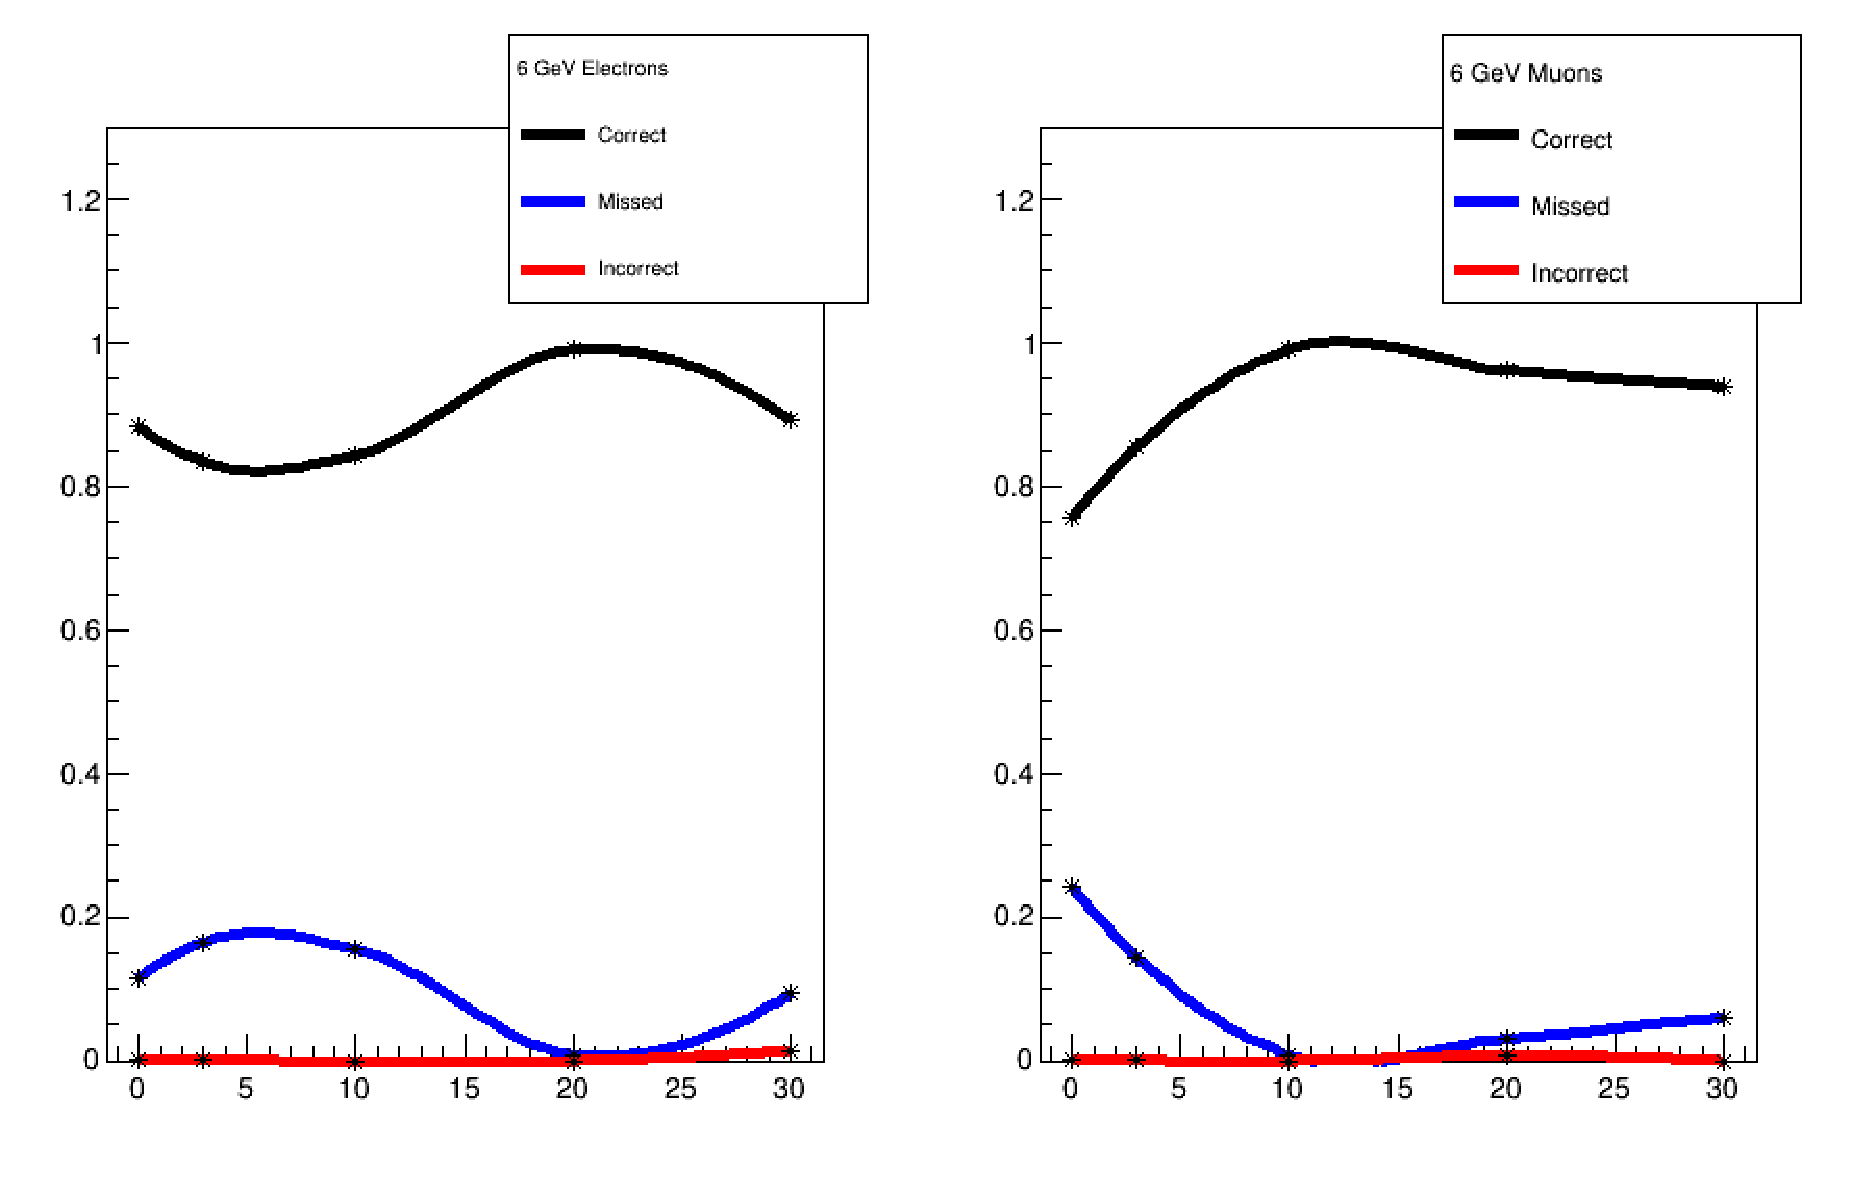
\includegraphics[width=0.8\textwidth]{disambigfractions_36.pdf}
\end{cdrfigure}

\subsection{Photon Detector Signal Reconstruction}

The photon detector signals are reconstructed in two steps.  First, a
hit finder identifies signals on an individual channel, looking for
peaks while account for noise and pedestal.  Each hit is assigned a
total integrated charge and a time associated with the first peak,
since the SiPM signals are asymmetric and multiple individual photons
may get grouped together into a single hit if they are close in time.
Second, a flash finder groups together hits from across multiple
photon detectors which are coincident in time (a ``flash'' being a
source of light in the detector like the scintillation from the
passage of a charged particle).  Each flash has a total integrated
charge determined from its constituent hits as well as a
two-dimensional position determined by a charge-weighted average of
the positions of the photon detectors.  Since the photon detectors all
sit in a single plane, only two dimensional position reconstruction is
possible.  Once a flash is reconstructed, it becomes a candidate $t_0$
for objects reconstructed by the TPC.  If only a single track or
shower is present in the detector near the time of the flash, the
association is clear, but if there are multiple overlapping tracks a
likelihood-based method associates a TPC object with its best matching
flash.


\subsection{TPC Hit Clustering}

After the hit-finding and disambiguation stages have completed, a series of 
pattern recognition algorithms are applied to the 2D hits in order to identify 
the tracks and showers produced by individual final-state particles in an event.
In Liquid Argon TPC detectors, the pattern recognition stage must perform 
two functions in order to reconstruct 3D particles from 2D hits:
(a) identify the patterns of hits within each two-dimensional view
that correspond to individual particles; (b) match up hits and trajectories
between views in order to reconstruct particles as three-dimensional objects.
The development of automated pattern recognition algorithms for Liquid Argon 
TPC detectors is a relatively new field, but several 2D and 3D algorithms
have been implemented, using a range of different techniques.
For example, the ``Fuzzy Cluster'' package is a suite of algorithms that
performs two-dimensional clustering of hits using several techniques developed 
outside of HEP~\cite{flameclustering}~\cite{pphtclustering}~\cite{Ester96adensity-based}.

A promising suite of pattern recognition algorithms, that provides fully 
automated reconstruction of 3D particle tracks and showers from 2D hits, 
is the PANDORA software development kit~\cite{Marshall:2013bda,Marshall:2012hh}.
PANDORA implements a highly modular approach to pattern recognition,
in which the final-state particles within an event are reconstructed using 
a large chain of focused algorithms, each designed to identify and handle
a specific event topology. The reconstruction chain begins with a 
series of 2D pattern recognition algorithms that group together hits 
into clusters based on their topology and spatial proximity.
The next stage of the chain is 3D track reconstruction, 
which uses a rank-three tensor to match up all possible combinations 
of 2D clusters between the $U$, $V$, and $Z$views, and group together 
the best-matched triplets or doublets of clusters. If necessary, 
2D clusters are modified to improve the consistency of the 3D event. 
Once the 3D track trajectories have been identified, 
a series of vertex-finding algorithms are applied to the event,
which reconstruct the neutrino interaction vertex by analyzing 
the 2D and 3D event topology. The remaining 2D clusters are then
used to reconstruct electromagnetic and hadronic showers,
first as extended 2D clusters, and then as 3D particles, 
using a similar procedure to 3D track reconstruction.
Finally, a neutrino event is formed by connecting together the 
reconstructed tracks and showers at the interaction vertex.


The PANDORA pattern recognition algorithms have been developed
using simulated neutrino interactions in the energy range 100\,MeV\,$-$\,25\,GeV.
Figure~\ref{fig:recoannexpandoraeventdisplays} shows some example events.
Figure~\ref{fig:recoannexpandoraefficiency} shows the efficiency for reconstructing
the leading final-state lepton in 5\,GeV $\nu_{e}$ CC and $\nu_{\mu}$ CC interactions,
plotted as a function of momentum using the MicroBooNE detector geometry.
In both samples, the reconstruction efficiency increases rapidly with momentum,
rising above 90\% at 500\,MeV and reaching approximately 100\% at 2\,GeV.
Figure~\ref{fig:recoannexpandoravertexresolution} shows the spatial resolution for
reconstructing the primary interaction vertex in 5\,GeV $\nu_{\mu}$ CC events,
projected onto the $x$, $y$ and $z$ axes. An estimate of the overall vertex 
resolution is obtained by taking the 68\% quantile of 3D vertex residuals, 
which yields 2.2\,cm (2.5\,cm) for $\nu_{\mu}$ CC ($\nu_{e}$ CC) events.


%\fixme{CLUSTERING/PANDORA FOR LBNO (TWO VIEWS), taken from LGUNA-LBNO deliverables document}

%For the dual-phase event reconstruction, where only two views are available,
%the PANDORA reconstruction uses a similar set of 2D algorithms but
%a modified 3D approach. 

Algorithms specific for reconstruction with two views, as is the case for the dual-phase detector design,
have been extensively developed as well. 
A preliminary 2D clustering is carried on similarly to what described above.
A first-pass hit clustering, using a nearest-neighbor algorithm and association algorithms is performed
for each projection. Then the primary vertex is identified based on the presumed beam direction and cluster positions and directions.
Redundant information from all readout views is used to constrain the vertex location.
Primary final-state particles (seed-clusters) are finally identified, based on cluster length and proximity to vertex,
and each of the remanining non-seed clusters is associated with existing seed-clusters so that 
all energy deposits from a single final-state particle are grouped together.
At the end of this process, clusters not directly related to the vertex, as ascertained either by pointing or position,
will be associated with clusters coming from the vertex which are in close proximity, 
as long as there is not another vertex-related cluster nearby. 
%Any remaining clusters far from the vertex will be removed, 
%since it is assumed that these are actually related to an original final state particle, but we have been unable to make the association.

The PANDORA reconstruction has been tested on charged current events generated by both $\nu_{e}$  and $\nu_{\mu}$  
considering the processes $\nu_{\ell}\to \ell+p$  and $\nu_{\ell}\to \ell+p+\pi^{+}$.
The neutrino energy distribution is simulated by means of a detailed beam flux simulation.
Particles produced in the neutrino interactions were then generated by taking GENIE output, 
selecting only events with matching final state topologies, 
and simulating these events using Qscan.
 The performance has been tested by using truth information to associate each final-state particle with up to one reconstructed cluster.
The quality of the neutrino event reconstruction 
is evalulated by performing hit-by-hit comparisons of simulated and 
reconstructed particles and calculating the following Monte-Carlo-based performance metrics: 
``completeness,'' which is defined as the fraction of hits generated by 
the true particle and contained in the reconstructed cluster, and  
``purity,'' which is defined as the fraction of hits in the reconstructed 
cluster that were deposited by the true particle.   The ``true particle'' is defined to be the
one that contributes the most hits to the reconstructed cluster.
Both the completeness and purity are found to be above 90$\%$ for 
particles with energies above 800\,MeV.
Figure~\ref{fig:recoannexpandoraperformancemetrics} shows purity and completeness metrics.

\begin{cdrfigure}[PANDORA event displays]{recoannexpandoraeventdisplays}
{Two-dimensional event displays showing PANDORA clustering of the hits generated by a 4~GeV $\nu_e$~CC event (left)
and a 18~GeV $\nu_\mu$ CC~event (right).  The color-coding of the hits is from the automatic cluster algorithms
but the particle ID labels have been added by hand.}
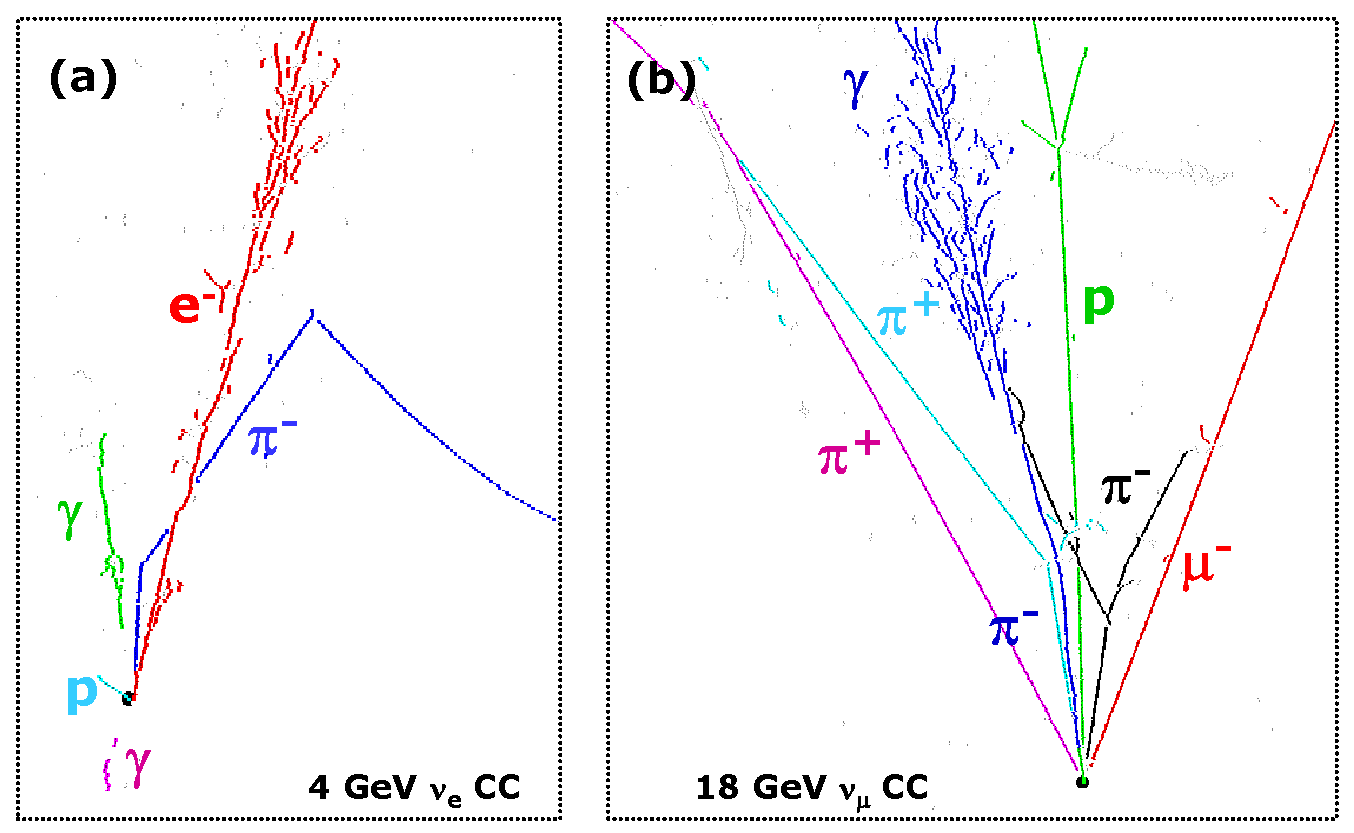
\includegraphics[width=\textwidth]{LArReco_EventDisplays_Take3.pdf}
\end{cdrfigure}

\begin{cdrfigure}[PANDORA reconstruction efficiency]{recoannexpandoraefficiency}
{Reconstruction efficiency of Pandora pattern recognition algorithms
 for the leading final-state lepton in 5\,GeV $\nu_{\mu}$ CC (left) and
 $\nu_{e}$ CC (right) neutrino interactions, plotted as a function of
 the lepton momentum. The reconstruction performance is evaluated
 using the MicroBooNE detector geometry. }
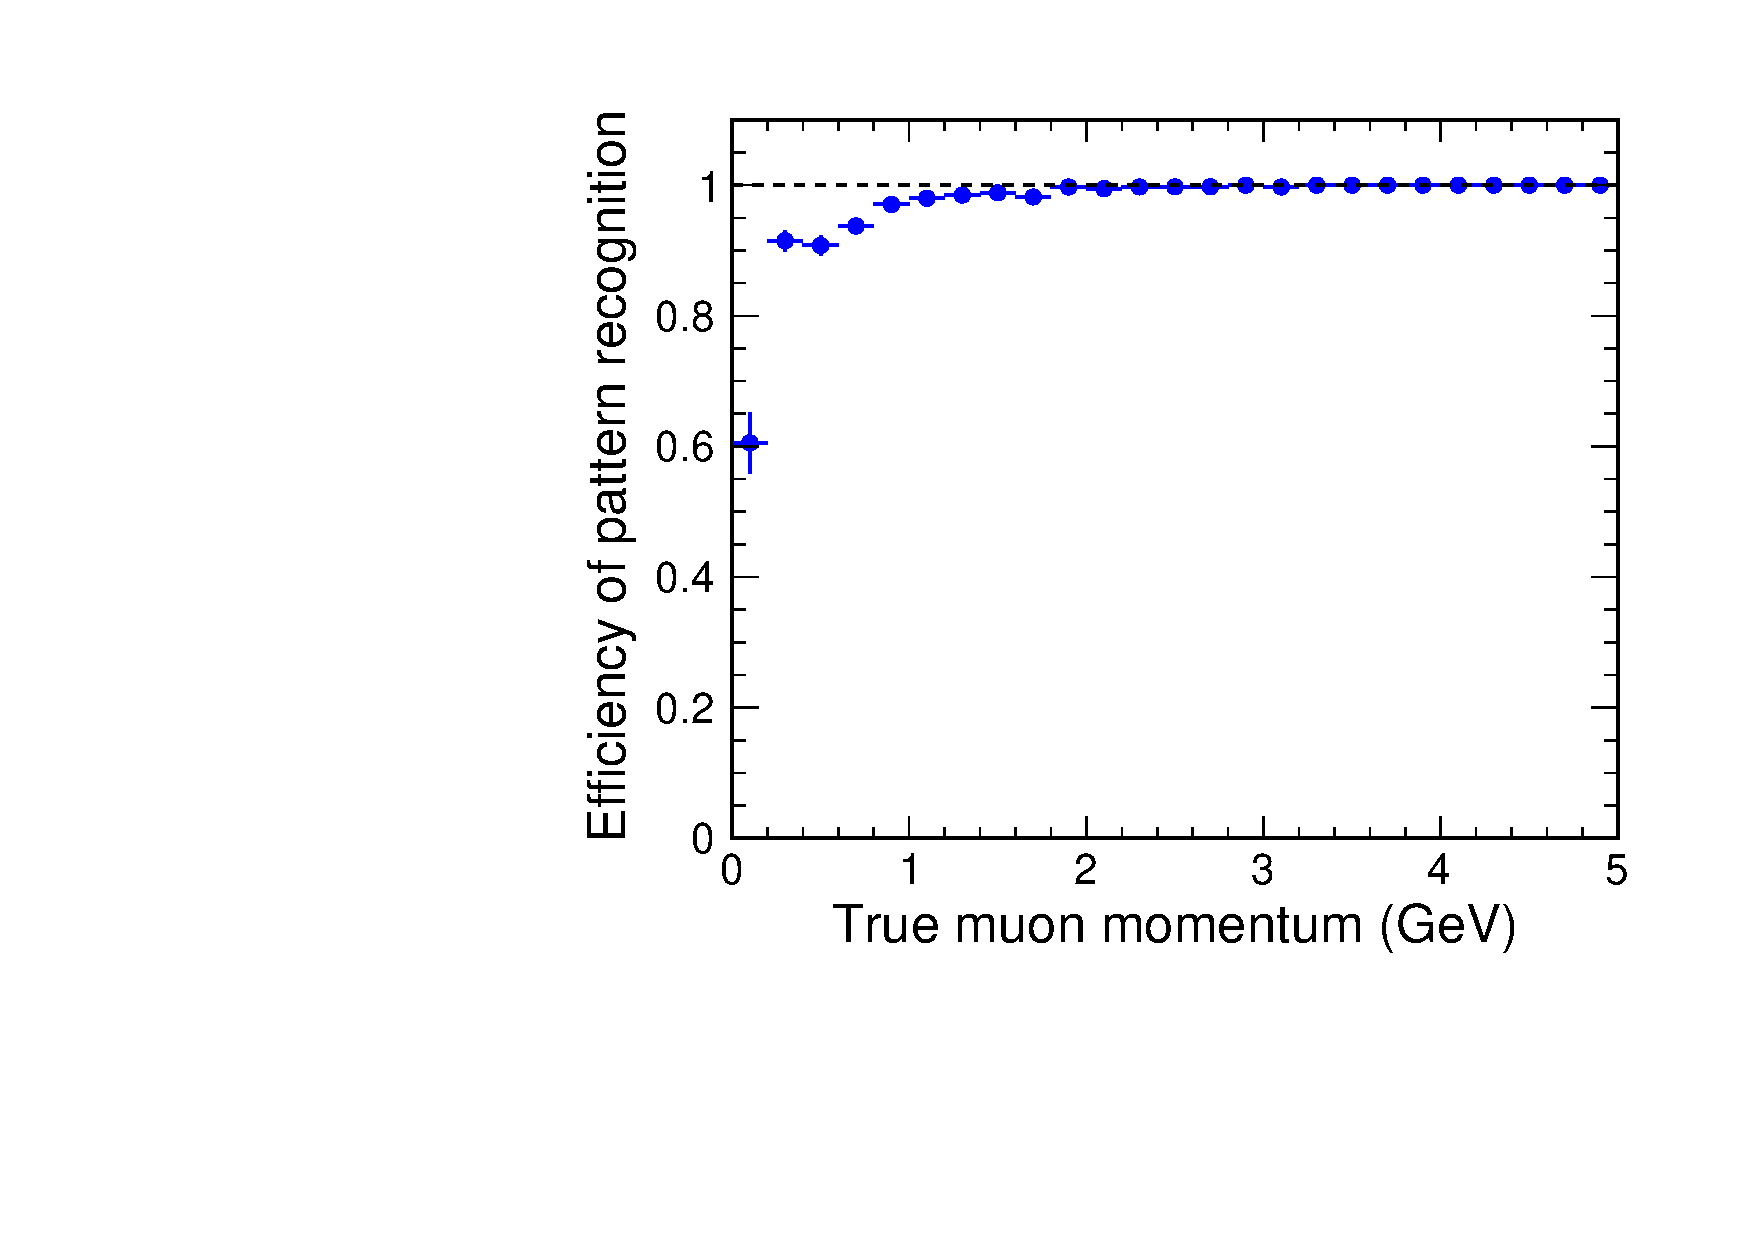
\includegraphics[width=0.49\textwidth]{pandora_uboone_efficiency_5GeV_numucc_annex.pdf}
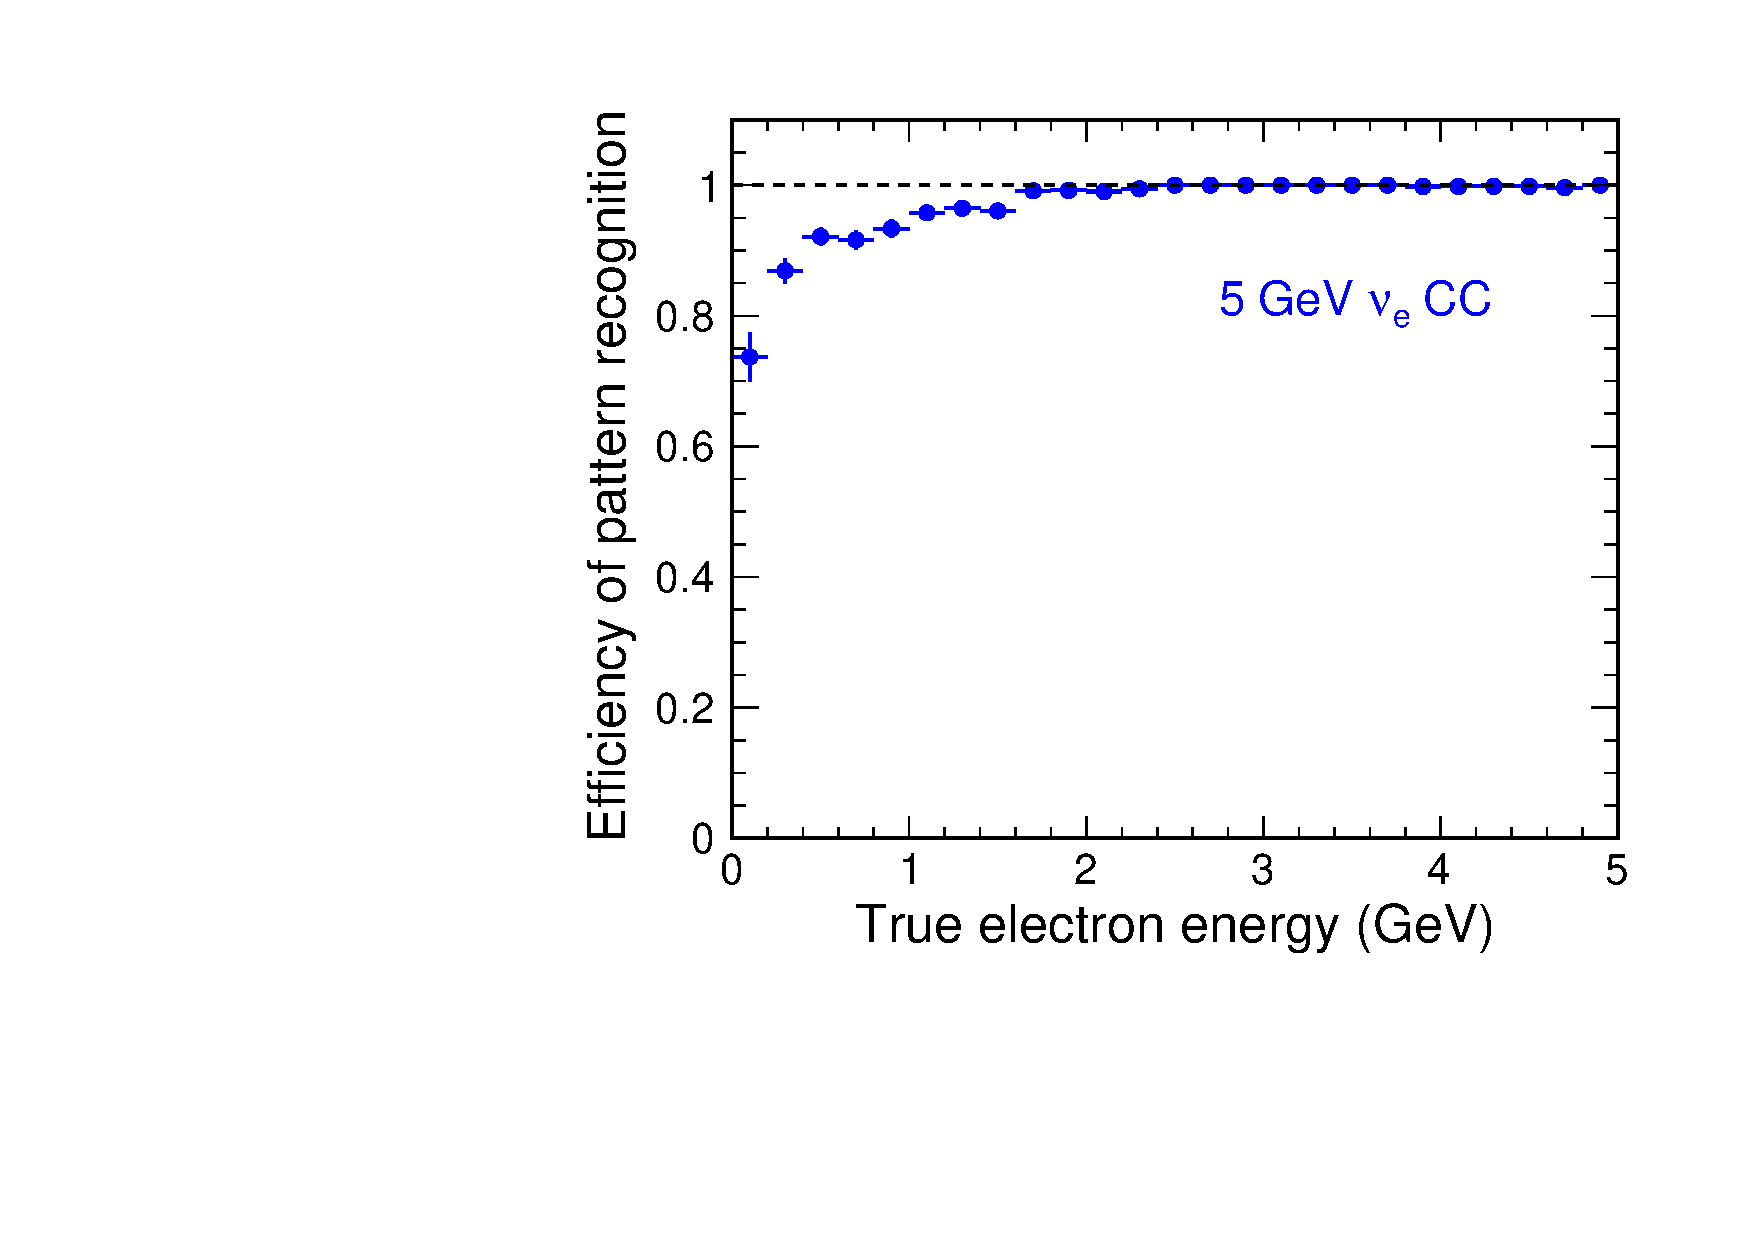
\includegraphics[width=0.49\textwidth]{pandora_uboone_efficiency_5GeV_nuecc_annex.pdf}
\end{cdrfigure}

\begin{cdrfigure}[PANDORA purity and completeness]{recoannexpandoraperformancemetrics}
{Distributions of purity and completeness for the PANDORA reconstruction of the cluster corresponding
to the leading lepton for a large sample of 5~GeV $\nu_\mu$~CC events (left) and a large sample
of 5~GeV $\nu_e$~CC events (right).}
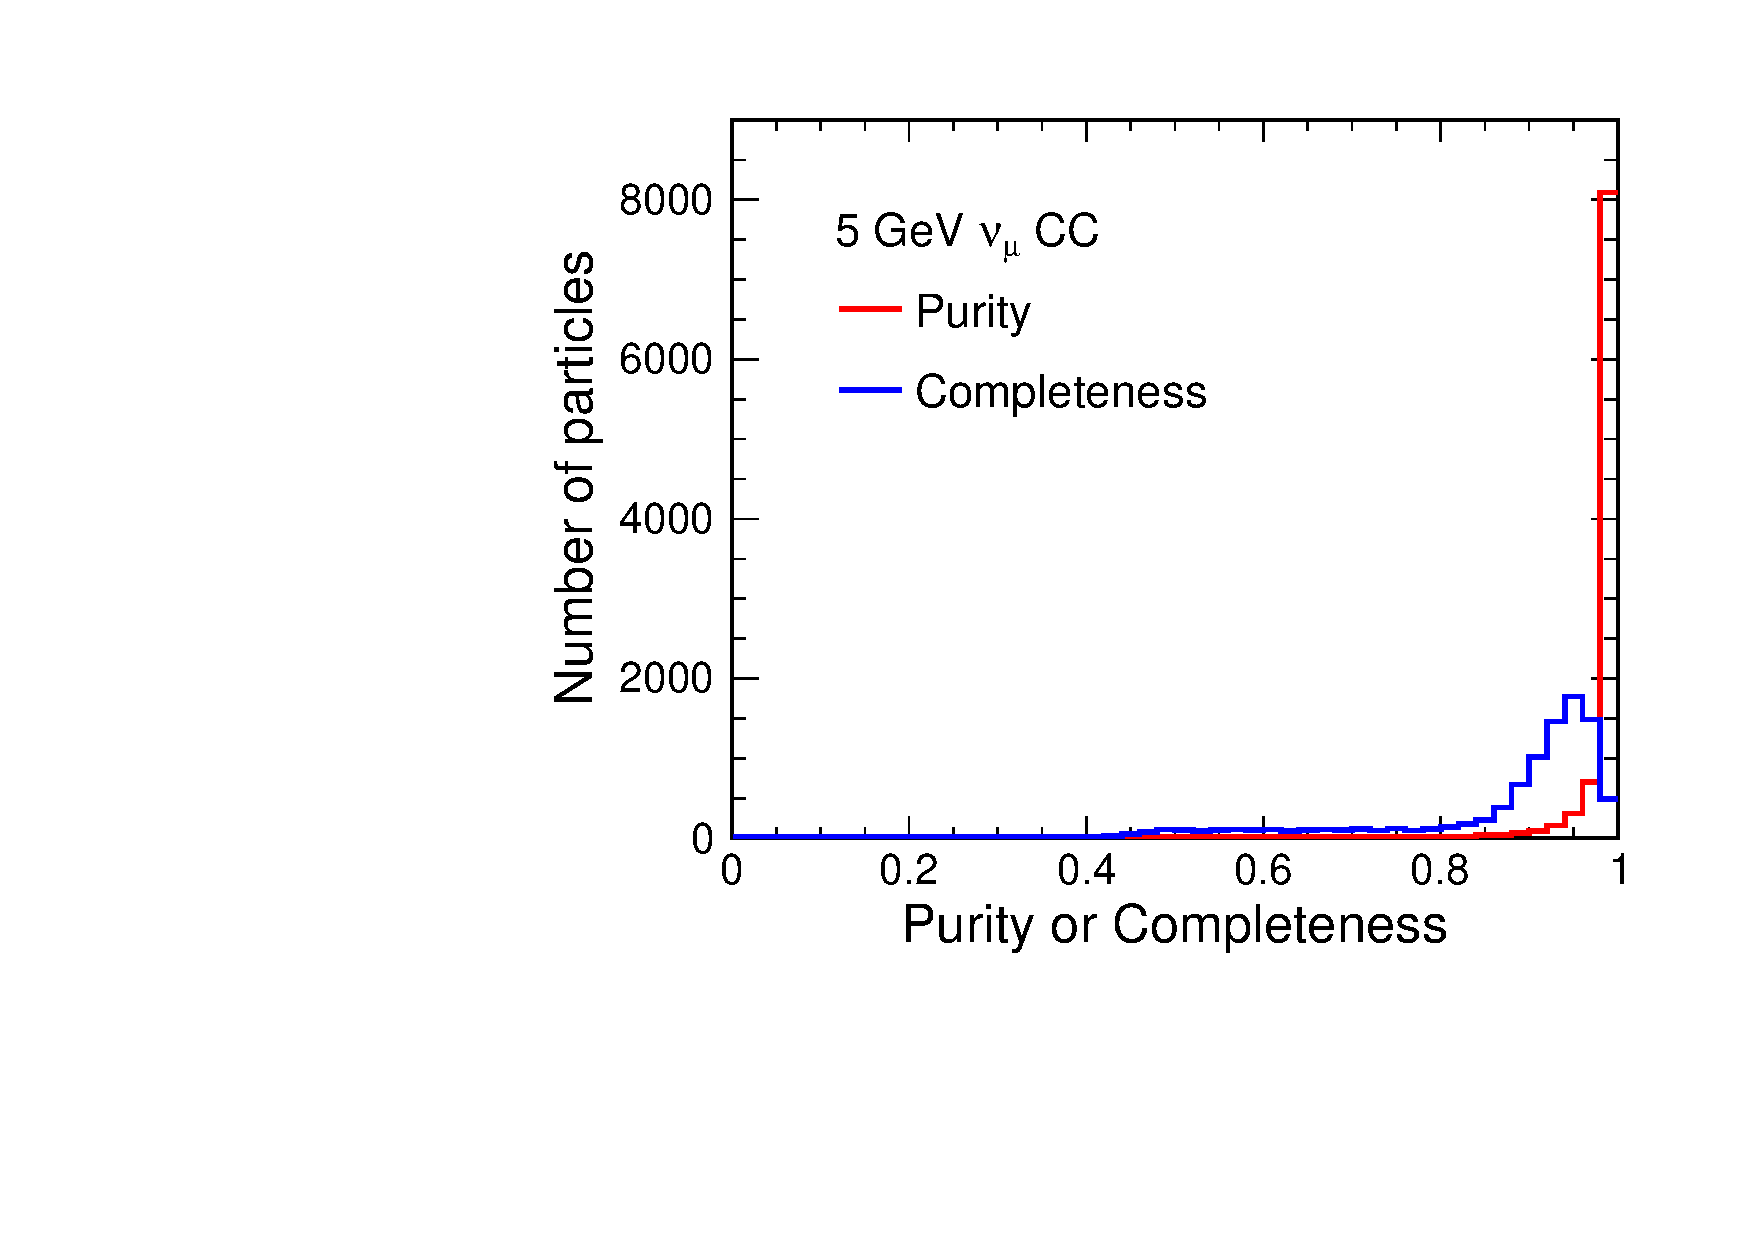
\includegraphics[width=0.49\textwidth]{pandora_uboone_purity_completeness_5GeV_numucc_annex.pdf}
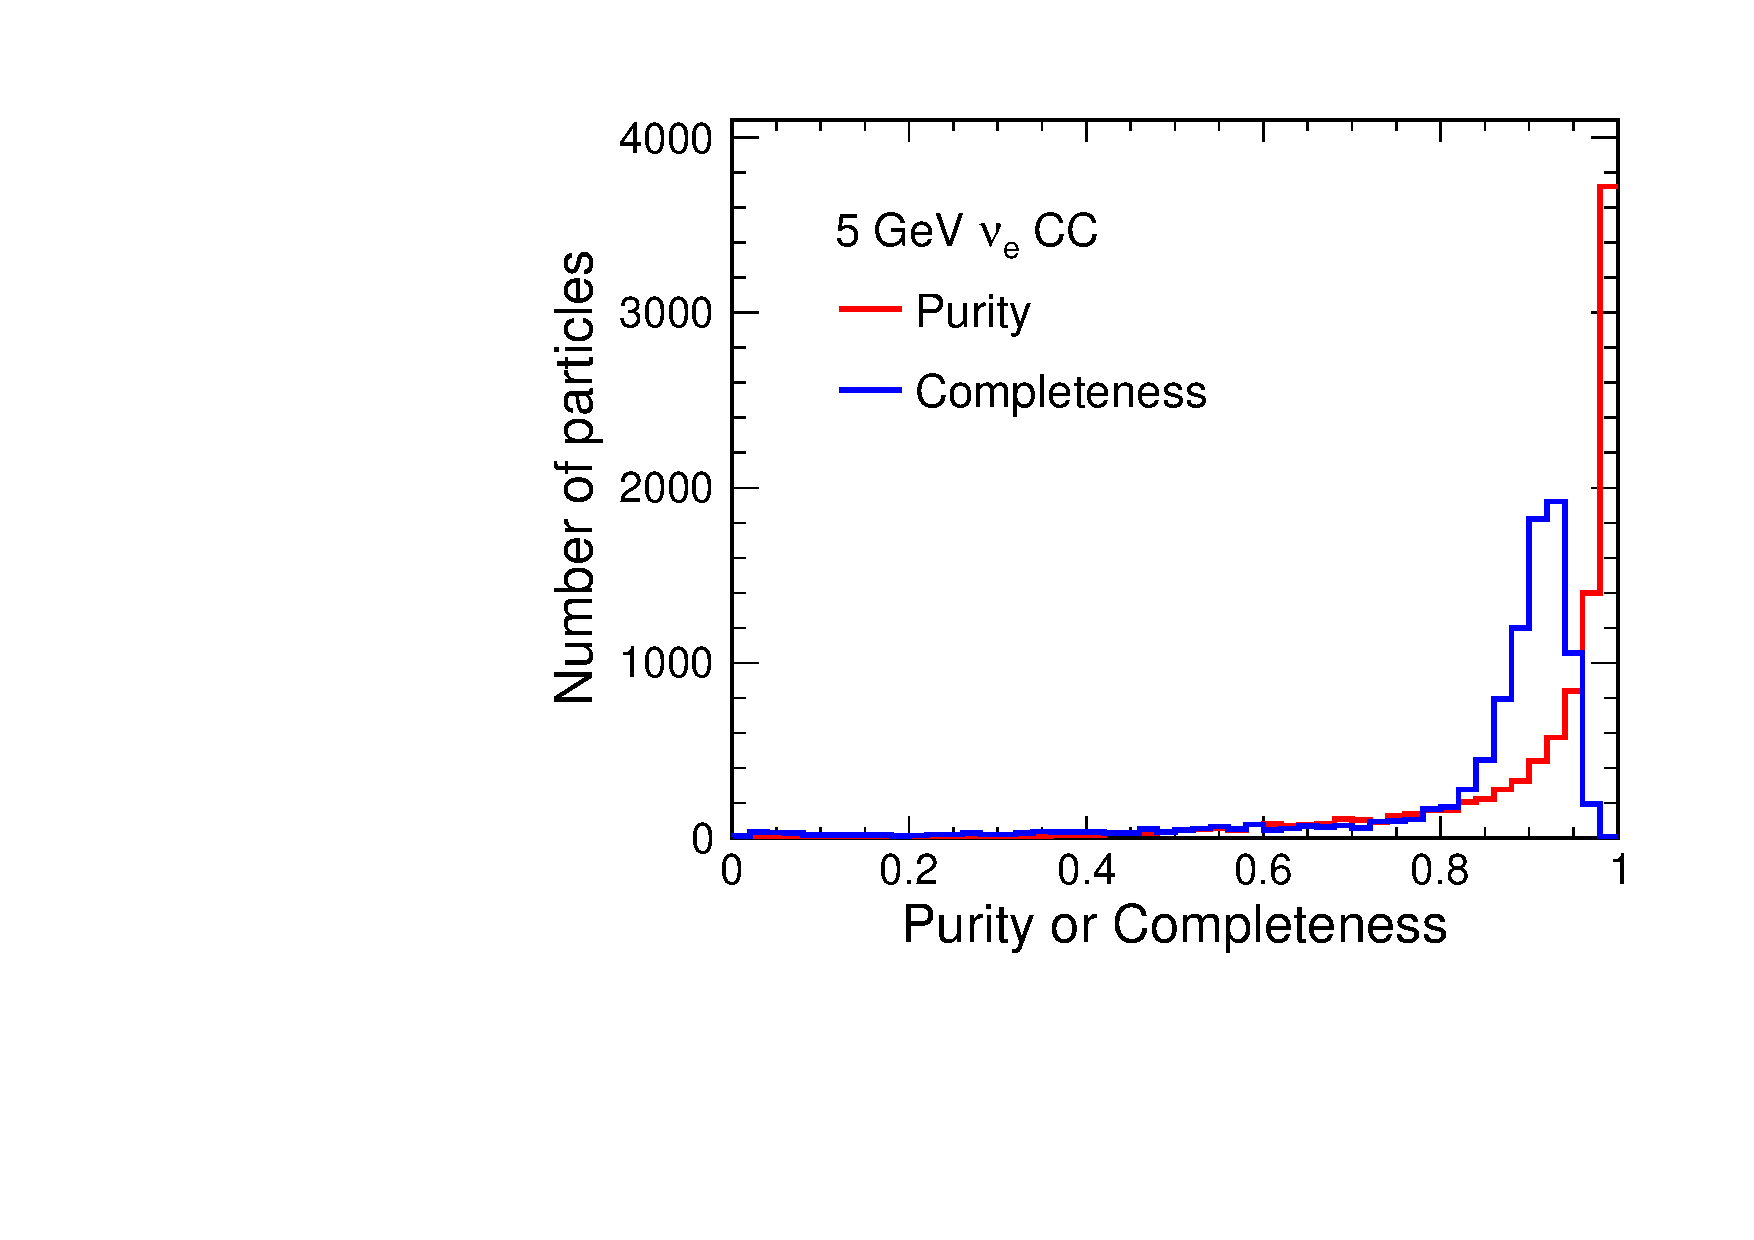
\includegraphics[width=0.49\textwidth]{pandora_uboone_purity_completeness_5GeV_nuecc_annex.pdf}
\end{cdrfigure}

\begin{cdrfigure}[PANDORA vertex resolution]{recoannexpandoravertexresolution}
{Distribution of 2D residuals between reconstructed and simulated interaction
 vertex for 5\,GeV $\nu_{\mu}$ CC (left) and$\nu_{e}$ CC (right) interactions in the MicroBooNE detector.
 The $x$ axis is oriented along the drift field, the $y$ axis runs parallel 
 to the collection plane wires, and the $z$ axis points along the beam direction.}
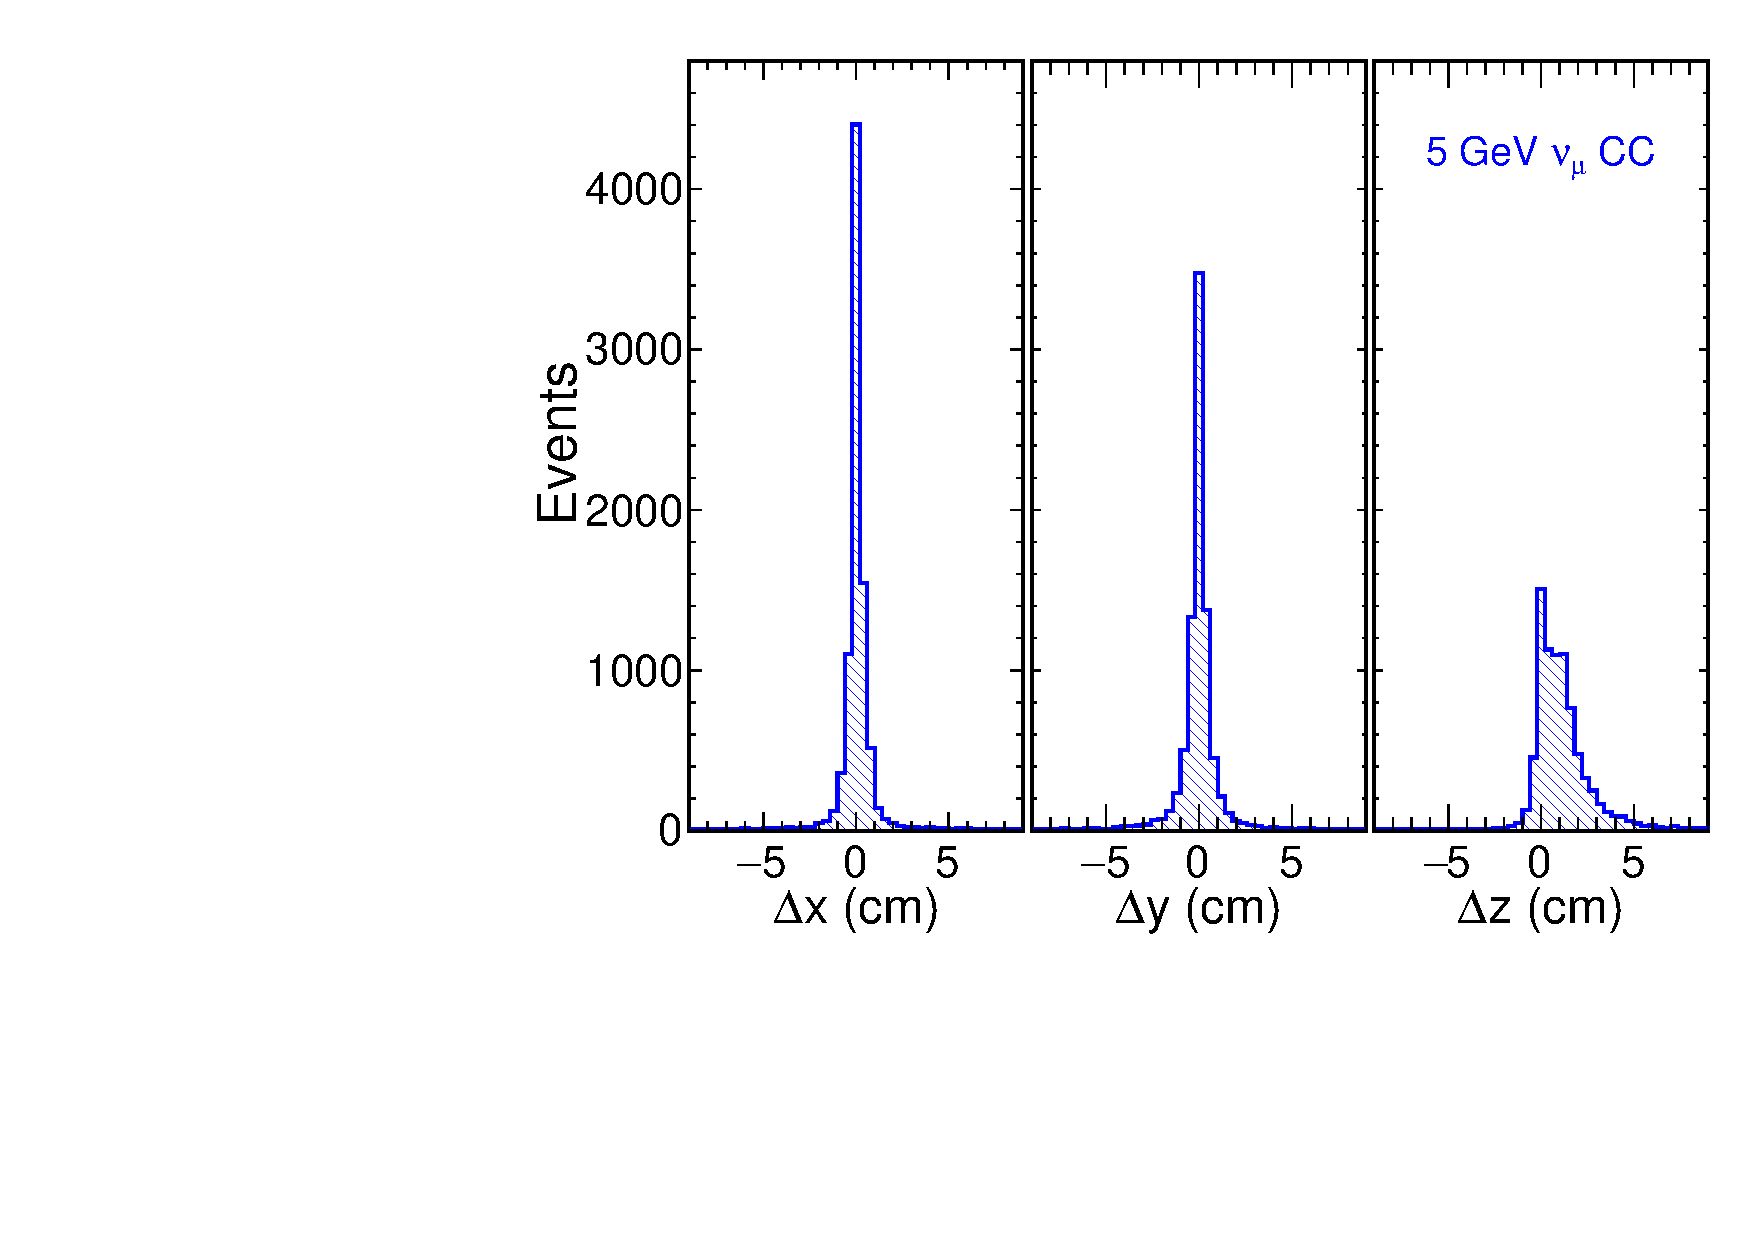
\includegraphics[width=0.49\textwidth]{pandora_uboone_vertex_resolution_numucc_annex.pdf}
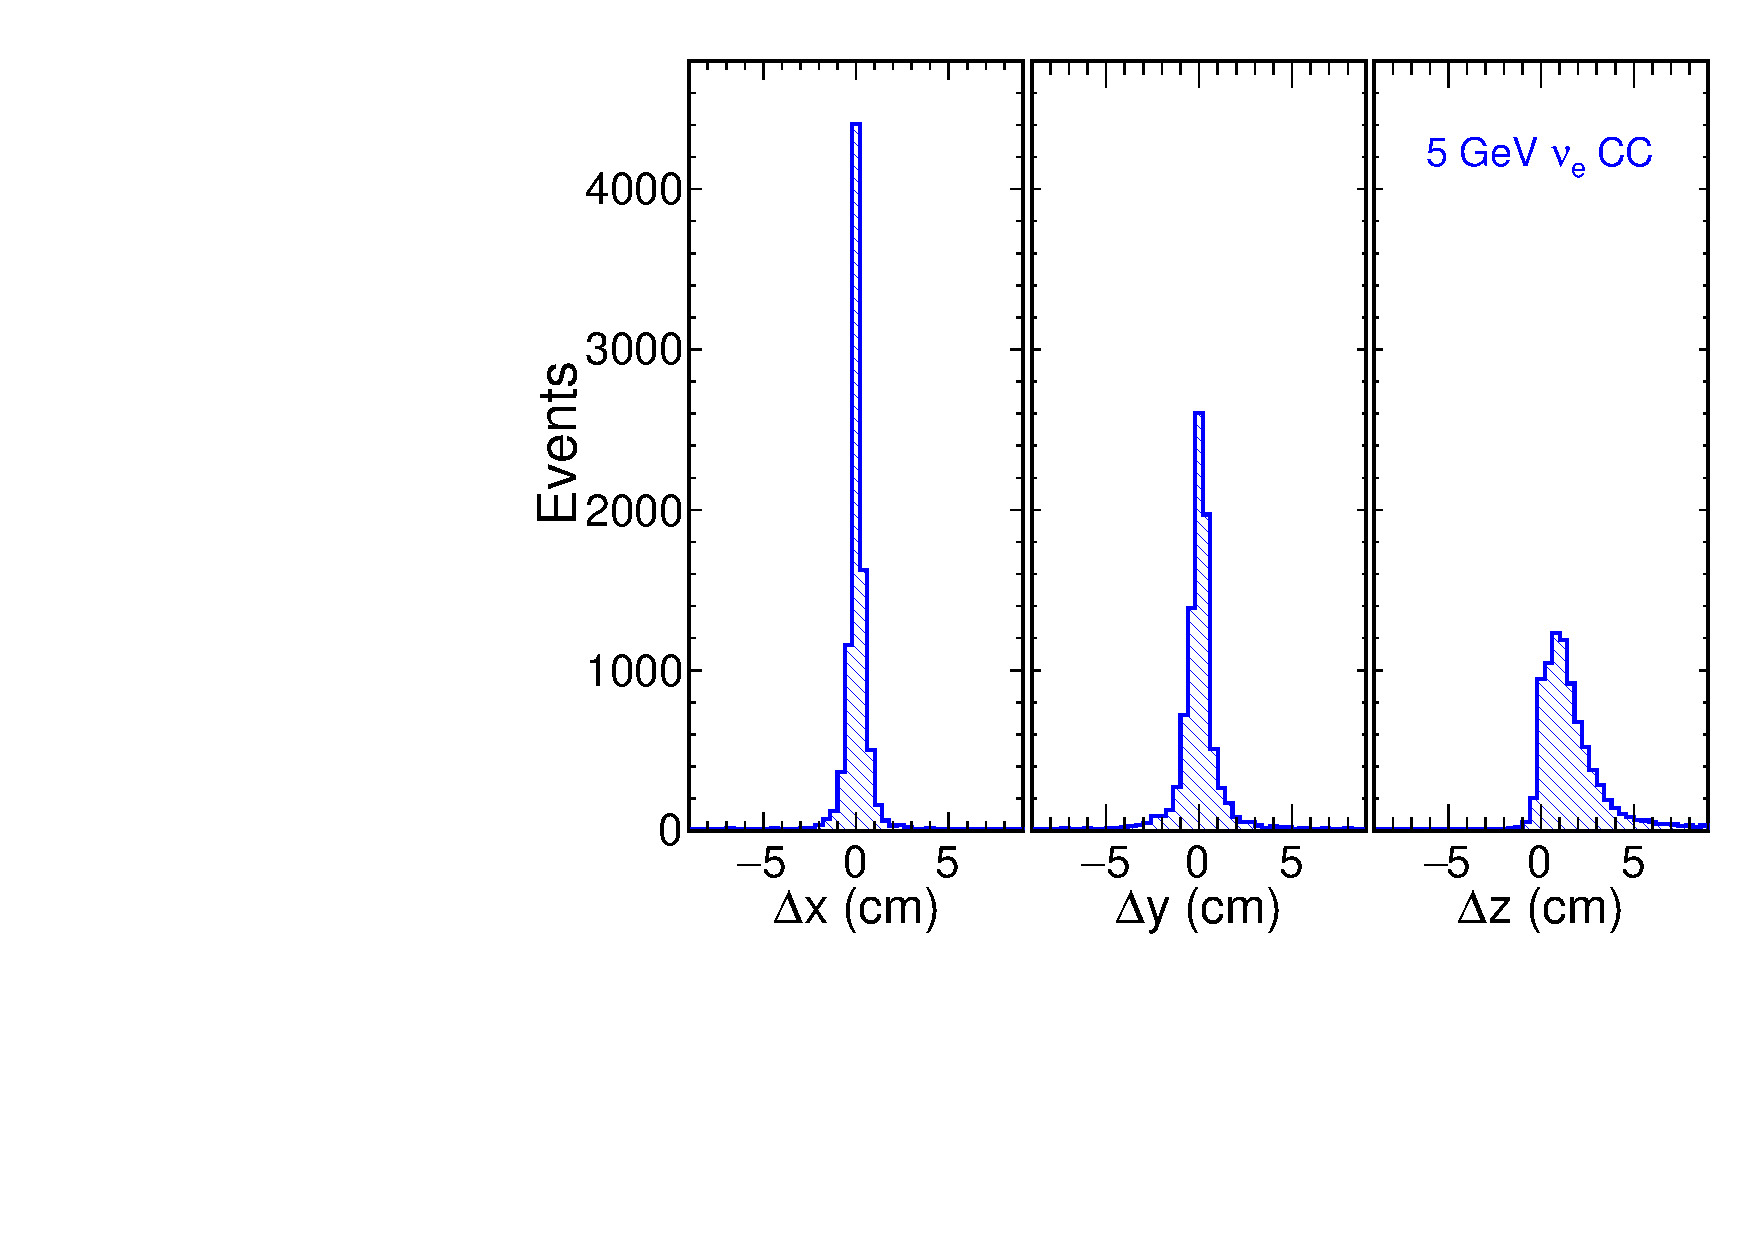
\includegraphics[width=0.49\textwidth]{pandora_uboone_vertex_resolution_nuecc_annex.pdf}
\end{cdrfigure}


\subsection{Track Fitting}

The track reconstruction algorithms in a liquid argon TPC is divided
into trajectory reconstruction and track parameter estimation.
Hits are the input data for track reconstruction.  Each hit represents a
one-dimensional measurement of a track (the drift time) on a
measurement surface defined by the charge drift direction and the
readout wire.  Hits from multiple views may be combined into
three-dimensional space points. Three dimensional track reconstruction
can proceed from space points or directly from hits.

The Kalman filter algorithm~\cite{kalman} has been widely used in high
energy physics for track reconstruction. The Kalman filter provides an
elegant mathematical solution to the problem of finding an optimal
track description from a collection of candidate measurements that are
hits or space points, especially in cases where the number of
measurements is much larger than the five parameters needed to specify
a track on a surface.  The Kalman filter can be used for both pattern
recognition and parameter estimation.
The Kalman filter technique has been applied
to 3D track reconstruction by ICARUS~\cite{Ankowski:2006ts}, and is being studied by MicroBooNE.
This technique incorporates the effects of multiple Coulomb scattering,
enabling a scattering-based estimate of the track momentum,
which is shown by ICARUS to be as good as $\Delta p/p \approx 10\%$, 
depending mainly on the track length~\cite{Ankowski:2006ts}.
The data from ICARUS have also been used to develop a precise
track reconstruction, which builds a 3D trajectory for each track by simultaneously
optimising its 2D projections to match the observed data~\cite{Antonello:2012hu}.
Another promising technique, based on the local principal curve algorithm, 
has been implemented in conjunction with the development of the 
dual-phase detector concept, and is shown to provide 
a precise reconstruction of two-particle event topologies~\cite{Back:2013cva,LAGUNA-LBNO-deliv},
including precise vertex reconstruction.
Figure~\ref{fig:recoannexlpcvertexresolution} shows vertex resolution plots for the dual-phase detector design.

\begin{cdrfigure}[Vertex reconstruction using local principal curves]{recoannexlpcvertexresolution}
{Spatial resolutions for the primary vertex reconstruction using local principal curves, separately in the $x$, $y$, and
$z$ directions, in a dual-phase detector.  The left-hand column shows the resolutions for CCQE $\nu_\mu\rightarrow \mu + p$
events, and the right-hand column shows the resolutions for CCQE $\nu_e\rightarrow e + p$ events.  The distributions
are fit to a sum of two Gaussians with equal means.  The effective width is quoted above each plot
as  $\sigma_1 + r* \sigma_2$, where $r$ is the ratio of amplitudes of the two Gaussian components. }
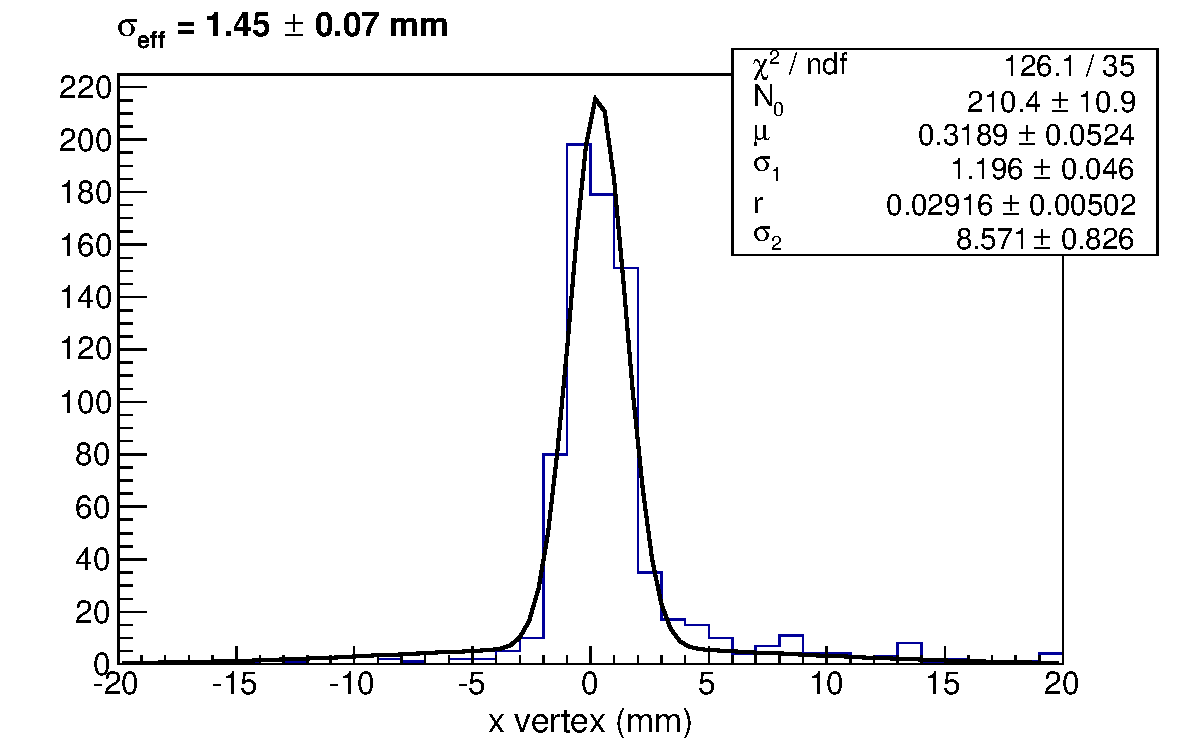
\includegraphics[width=0.33\textwidth]{barker_vertex_numuccqe_x_annex.pdf}
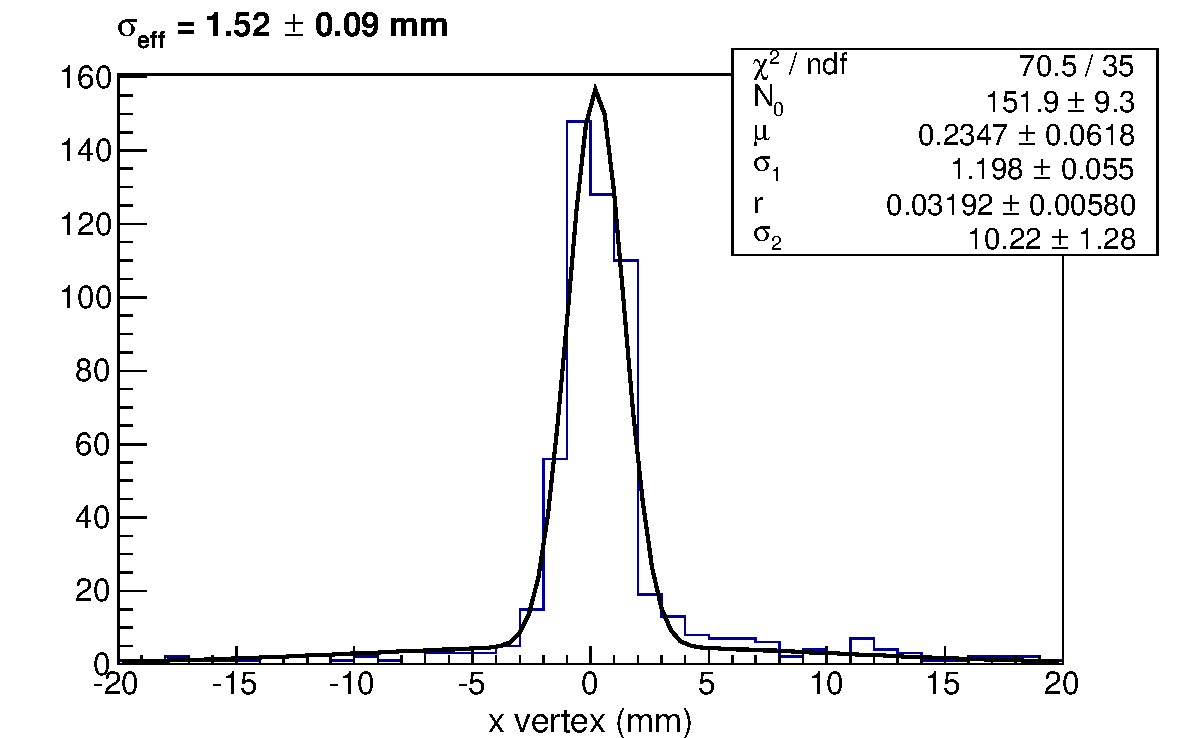
\includegraphics[width=0.33\textwidth]{barker_vertex_nueccqe_x_annex.pdf}
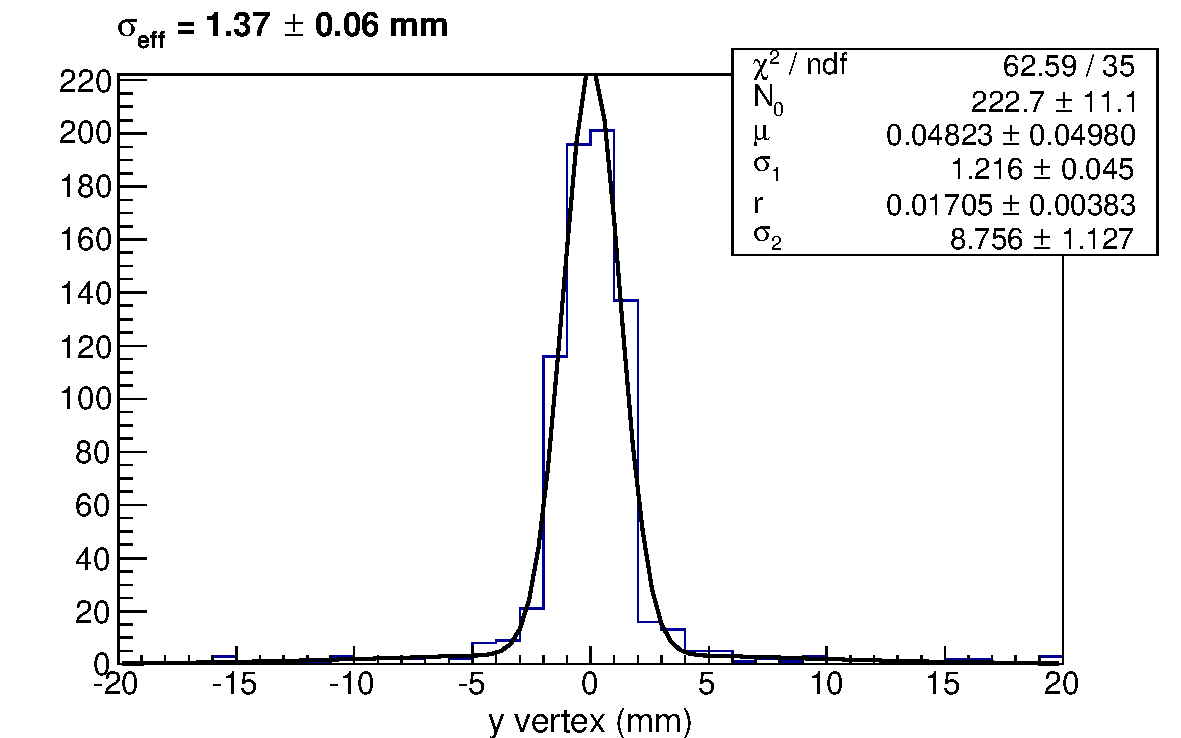
\includegraphics[width=0.33\textwidth]{barker_vertex_numuccqe_y_annex.pdf}
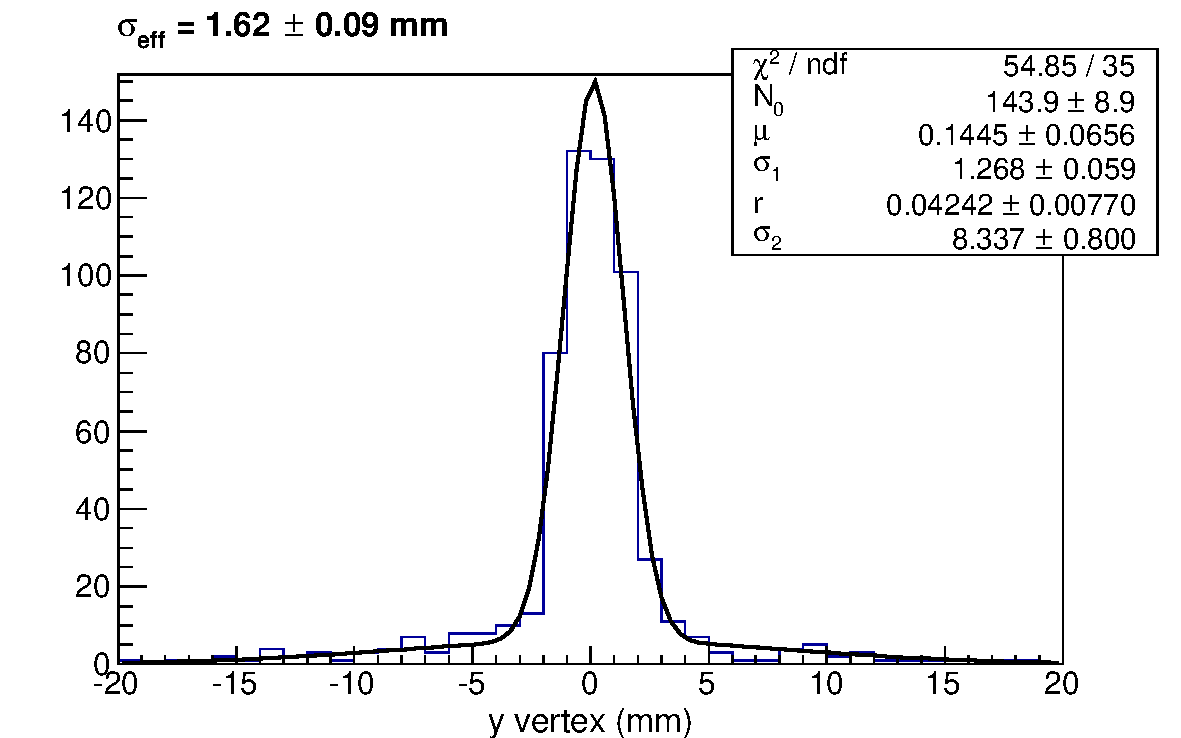
\includegraphics[width=0.33\textwidth]{barker_vertex_nueccqe_y_annex.pdf}
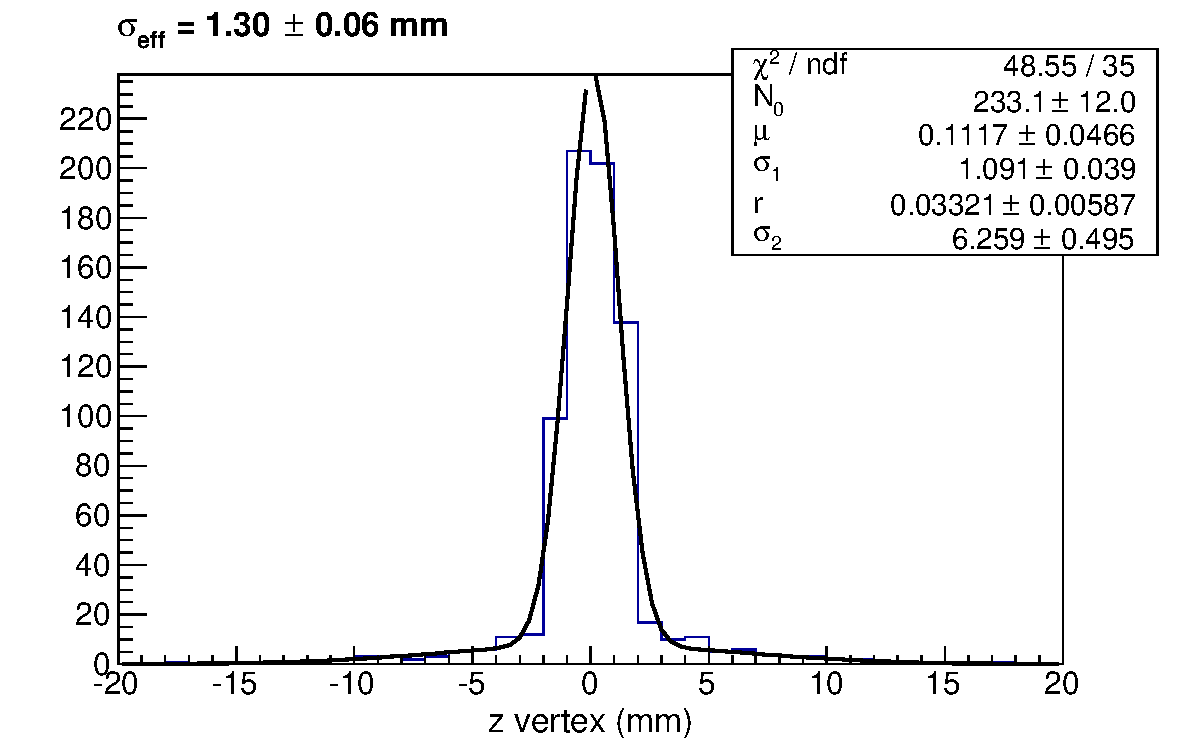
\includegraphics[width=0.33\textwidth]{barker_vertex_numuccqe_z_annex.pdf}
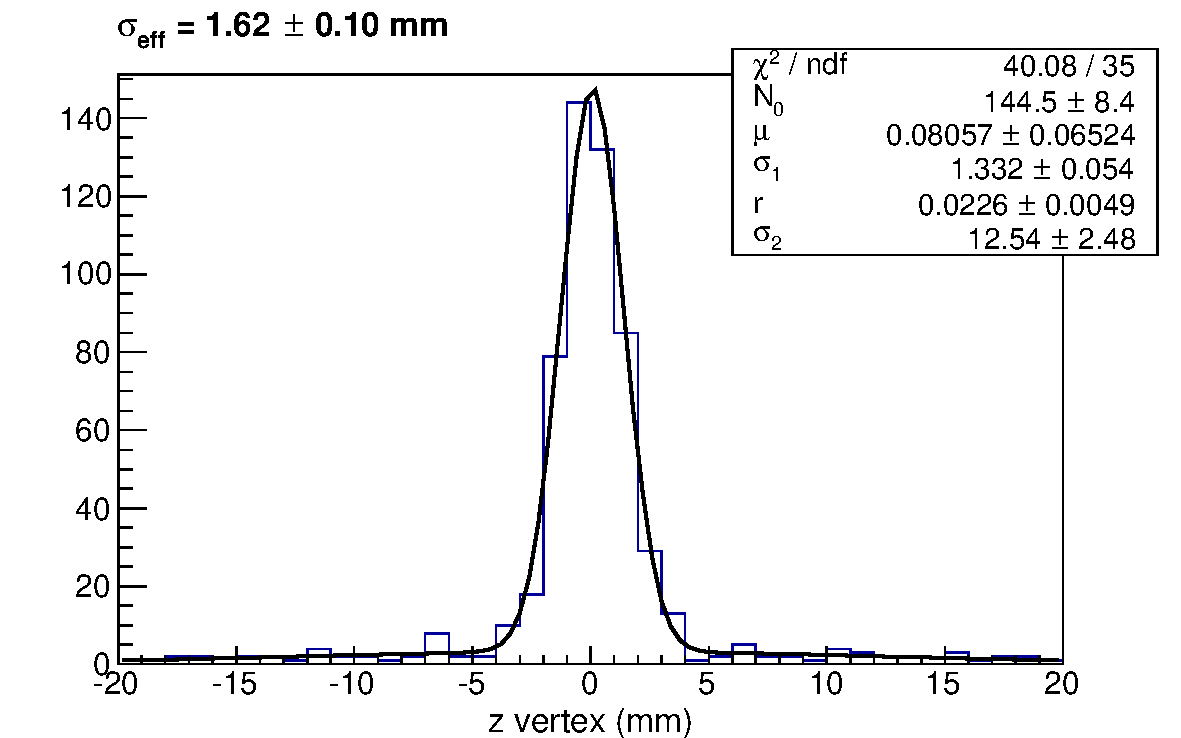
\includegraphics[width=0.33\textwidth]{barker_vertex_nueccqe_z_annex.pdf}
\end{cdrfigure}

%%%% MAYBE TOO MUCH DETAIL FOR CDR 

%The measurement surfaces in liquid argon TPCs intersect, which
%means there is no predetermined order in which the measurement
%surfaces should be visited.  To prevent back-and-forth tracking, which
%would overestimate propagation noise, such as multiple Coulomb
%scattering, the LArSoft Kalman filter chooses the measurement
%surfaces associated with one view as primary, and visits these
%surfaces in their natural predetermined order.  Hits from views other
%than the primary view are added to the track by treating the
%propagation from the track surface to the non-parallel hit measurement
%surface as part of the measurement function.  This measurement
%propagation is always done using a linear approximation as is the
%measurement function, and is done without propagation noise.

%The LArSoft Kalman filter does not use a branching track model. Hit
%selection for the LArSoft Kalman filter is implemented such that at
%each measurement surface, the filter accepts either zero or one
%hit. 

%If the Kalman filter assigns the wrong hit to a track, the track may follow
%the wrong road (e.g. a delta ray), or the track may otherwise end
%prematurely.  Fixing broken tracks relies on a track-stitching
%algorithm that runs after the initial Kalman filter reconstruction.

\subsection{Shower Measurement}

%%%%% Section taken from the LArSoft NIM article -- to rephrase

The electromagnetic shower algorithms have two
steps. The first is a post-clustering stage which examines the
existing clusters in terms of their 2D parameters to determine whether
the clusters are shower-like or track-like. 
The selected shower-like clusters are examined to assign starting points,
directions and angles in the wire-time plane. The second step is 
3D shower reconstruction, which
matches the 2D clusters between views in order to obtain 3D shower axes and start points.
These 3D parameters allow the calculation of the shower energies and charge
depositions at the starts of the showers, which are used in particle
identification. 

%\fixme{Can we say something about current status or performance?} -- Not really with DUNE
% would have to borrow something from MicrBooNE or ICARUS.

\subsection{Calorimetry}


As charged particles traverse a volume liquid argon, they deposit
energy through ionization and scintillation. It is important to
measure the energy depotion as it provides information on the particle
energy and and helps to identify what type of particle it is. The algorithm for reconstructing the ionization
energy in LArSoft is optimized for line-like tracks and is being
extended to showers. 
For each hit on a reconstructed track, the hit area or amplitude, in ADC counts, is
converted to the charge $Q_{\rm{det}}$, in fC units, on the wire using an
ADC to fC conversion factor.  This factor is to be calibrated either {\it in situ} with muons or with
test-stand measurements. To account for the charge loss along the drift due to
impurities, a first correction is applied to $Q_{\rm{det}}$ to to account for the finite
electron lifetime.  We define $Q_{\rm{free}}$ as the free charge after recombination
and before reattachment, and is given by  $Q_{\rm{free}} = Q_{\rm{det}}/e^{-t/\tau_{e}}$, where
$t$ is the electron drift time for the hit and $\tau_{e}$ is the
electron lifetime measured by the muons or purity monitors. The charge
$Q_{\rm{free}}$ is divided by the track pitch $dx$, which is defined as the
dot production of track direction and the direction normal to the wire
direction in the wire plane, to get the $dQ_{\rm{free}}/dx$ for the
hit. Finally, to account for charge loss due to recombination, also
known as ``charge quenching,'' a second correction is applied to
convert $dQ_{\rm{free}}/dx$ to $dE/dx$ based on the modified box model
\cite{Thomas:1987zz} or Birks's model\cite{Birks:1964zz}. The total energy
deposition from the track is obtained by summing the $dE/dx$ from each
hit: $\sum\limits_{i}^{\rm{all\ hits}}(dE/dx)_{i}\cdot dx_{i}$.

%first part same for Qscan (quenching, charge loss)
%
%leave what follow commented for the moment
%In the case of double phase LAr TPC events, 
%the energy scale parameters have been estimated, independently of the actual inputs to the Monte Carlo, using particle gun events. 
%Particles were generated at a range of energies, and the
%measured hit energies summed.
%This approach motivated by the fact that energy deposition profiles vary between particle types, 
%the quenching factor, and therefore the energy scale, will be different depending on the 
% cluster. In principle, the quenching scale should also depend on the particle energy, but this dependence is seen to be small.


\subsection{Particle Identification}

If the incident particle stops in the LArTPC active volume, the energy
loss, $dE/dx$, as a function of the residual range ($R$), the path
length to the end point of the track, is used as a powerful method for
particle identification. There are two methods in LArSoft to determine
particle species using calorimetric information. The first method
calculates four $\chi^{2}$ values for each track by comparing measured
$dE/dx$ versus $R$ points to the proton, charged kaon, charged pion
and muon hypotheses and identifies the track as the particle that
gives the smallest $\chi^{2}$ value. The second method calculates the
quantity ${\rm{PIDA}} = <A_{i}> = <(dE/dx)_{i}R_{i}^{0.42}>$ \cite{Thomas:1987zz},
which is defined to be the average of $A_{i} =
(dE/dx)_{i}R_{i}^{0.42}$ over all track points, indexed by $i$, where the residual
range $R_{i}$ is less than 30 cm. The particle species can be
determined by making a selection on the PIDA value.

Another method was developed for the ICARUS reconstruction software
and may be incorporated with LArSoft. The vector of probabilities $p_i$
of each considered particle hypothesis ($p$, $K^\pm$, $\pi^\pm$, $\mu^\pm$,
or none of the above as the fifth hypothesis) is calculated for each
measured point $q_j = (dQ/dx; R)$, where $dQ$ is the calorimetric
measurement (correction for the recombination effect is not
required). The probabilities $p_i$ are obtained as outputs from a neural
network trained on a set of $(dQ/dx; R)$ points calculated for
reconstructed MC tracks. The final probabilities of each PID
hypothesis are calculated as products of mutually independent $p_i$ for
all points along the tested track (similarly to the PIDA algorithm, the last 30~cm
of the track is used). The same neural network outputs as functions of the
$dQ/dx$ and $R$ variables are used to test the hypothesis if the incident
particle is actually stopping.

The $dE/dx$ information is also used for $e-\gamma$
discrimination, a method complementary to the topological
discrimination.  A cascade produced by an electron is
expected to have a $dE/dx$ characteristic of a single minimum-ionizing particle (MIP)
in its initial part, before the shower develops. A cascade produced by a gamma
converting to an $e^+e^-$ pair is expected to have a two-MIP $dE/dx$ in its initial part. 
An algorithm proposed for the reconstruction of the initial part of the cascade is
based on Ref.~\cite{Antonello:2012hu}. A straight 3D segment with one
endpoint fixed at the primary vertex position is created.  The position
of the other endpoint of the segment is optimized to minimize distances
between the segment 2D projections and hits of clusters corresponding
to the cascade initial part. The 3D length used to measure $dE/dx$ is at
most 2.5~cm. The method does not require explicit association of hits
between 2D planes and is efficient also for a low number of
hits.  There are, however, event topologies in which the $dE/dx$
reconstruction fails. The cascade initial part projection can be too
short or it may be shadowed by the cascade itself if the cascade develops
in a cone around an axis parallel to the readout wires. Such configurations may
prevent the spatial reconstruction or may cause inaccurate $dE/dx$
measurements if they occur for the collection plane, which is used for charge
measurement. The efficiency of electron selection versus gamma
rejection in the isotropic distribution of cascades is illustrated in
Fig.~\ref{fig:egammasepvssnratio} (simulation prepared with FLUKA~\cite{FLUKA1,FLUKA2} for
the single-phase configuration as foreseen for the far detector). The curves in the
figure are obtained for varying the cut on the reconstructed $dE/dx$
value. The effect of unfavorable spatial orientations of the cascade can be
practically eliminated if the charge measurement can be performed also
with the induction planes. Another source of inefficiency in this method
occurs mainly in the low energy range, and is related to the
contribution of cascades from gammas undergoing Compton scattering, which 
produces a single MIP $dE/dx$, or gammas that convert into $e^+e^-$ pairs
with a large asymmetry in their energies, which produces a 
flat distribution in $dE/dx$ between single and double MIP rates. 
The dependence on the cascade energy of the performance of $e-\gamma$ separation using $dE/dex$
is illustrated in Fig.~\ref{fig:egammasepvsenergy}.

\begin{cdrfigure}[Performance of $dE/dx$-based $e-\gamma$ separation vs S/N]{egammasepvssnratio}
{Peformance of the $e-\gamma$ separation algorithm using the ionization density of the
initial part of the EM shower, as functions of the assumed signal to noise ratio S/N.  Left
panel:  photon rejection vs. electron efficiency for all events.  Right panel:  the same,
but only for events with sufficient hits in the initial part of the shower to reconstruct
it well (see text).}
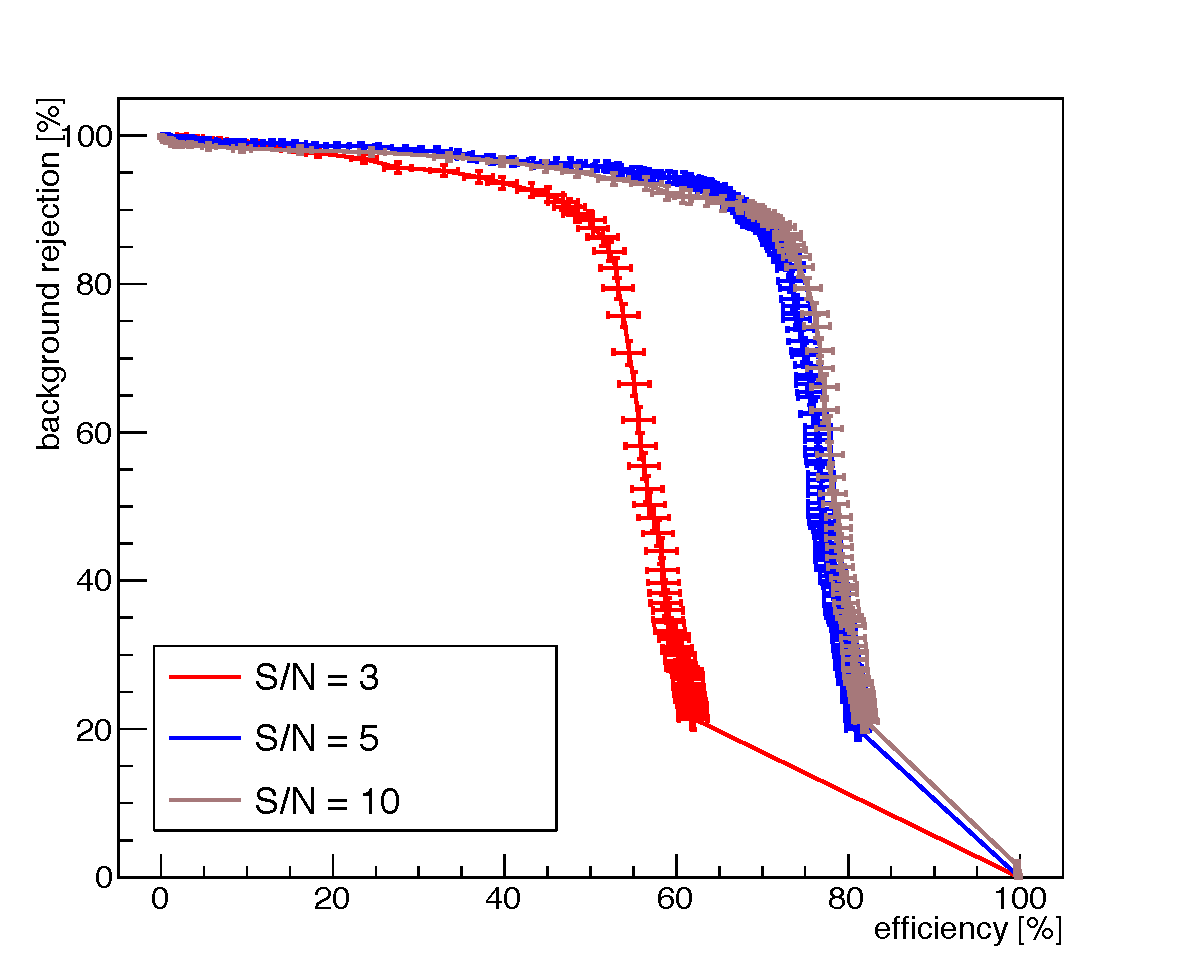
\includegraphics[width=0.49\textwidth]{annex_sn_allnorm.pdf}
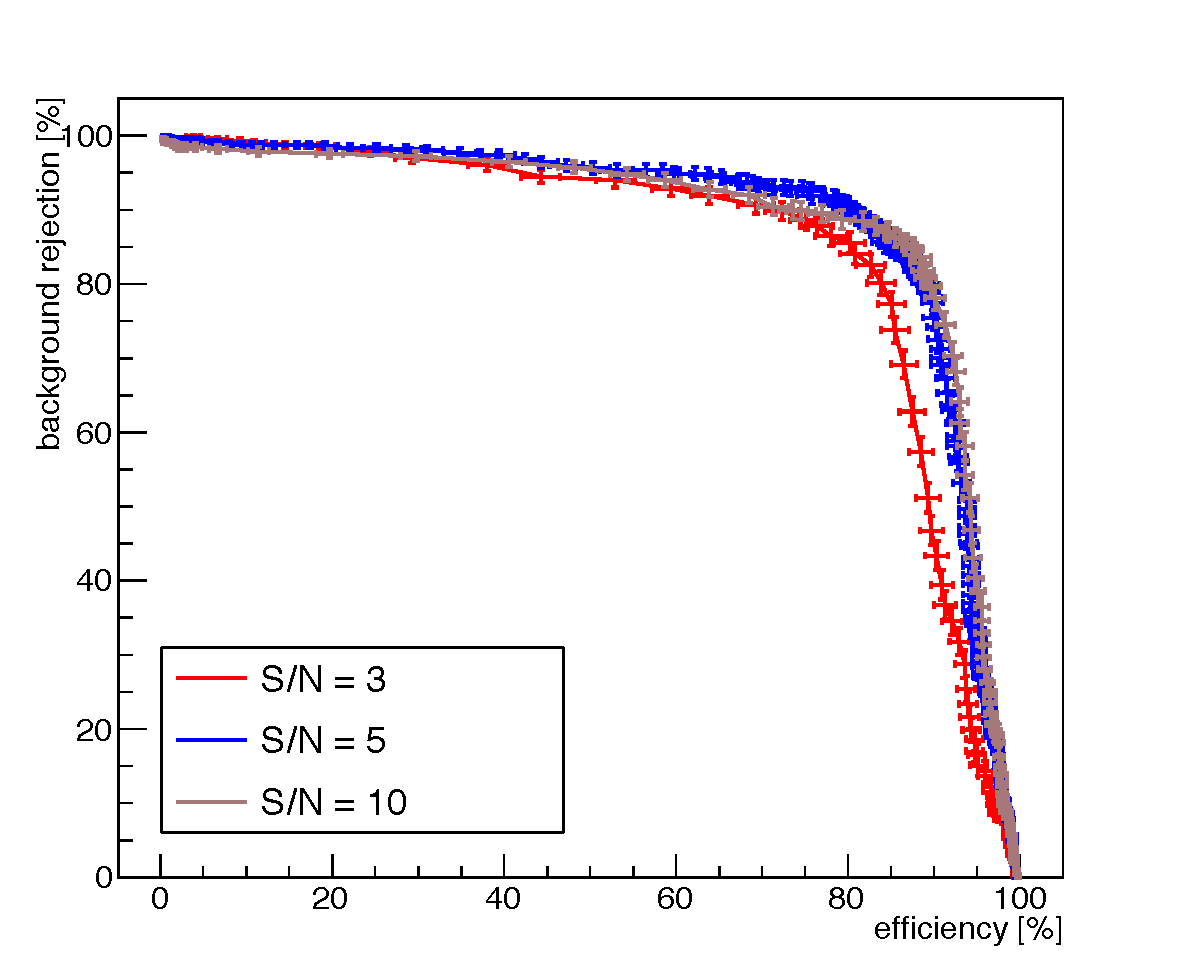
\includegraphics[width=0.49\textwidth]{annex_sn_recnorm.pdf}
\end{cdrfigure}

\begin{cdrfigure}[Performance of $dE/dx$-based $e-\gamma$ separation vs Energy]{egammasepvsenergy}
{Peformance of the $e-\gamma$ separation algorithm using the ionization density of the
initial part of the EM shower, as functions of the energy of the electron or photon.  Only
events with well-reconstructed initial portions of the shower are included (see text).}
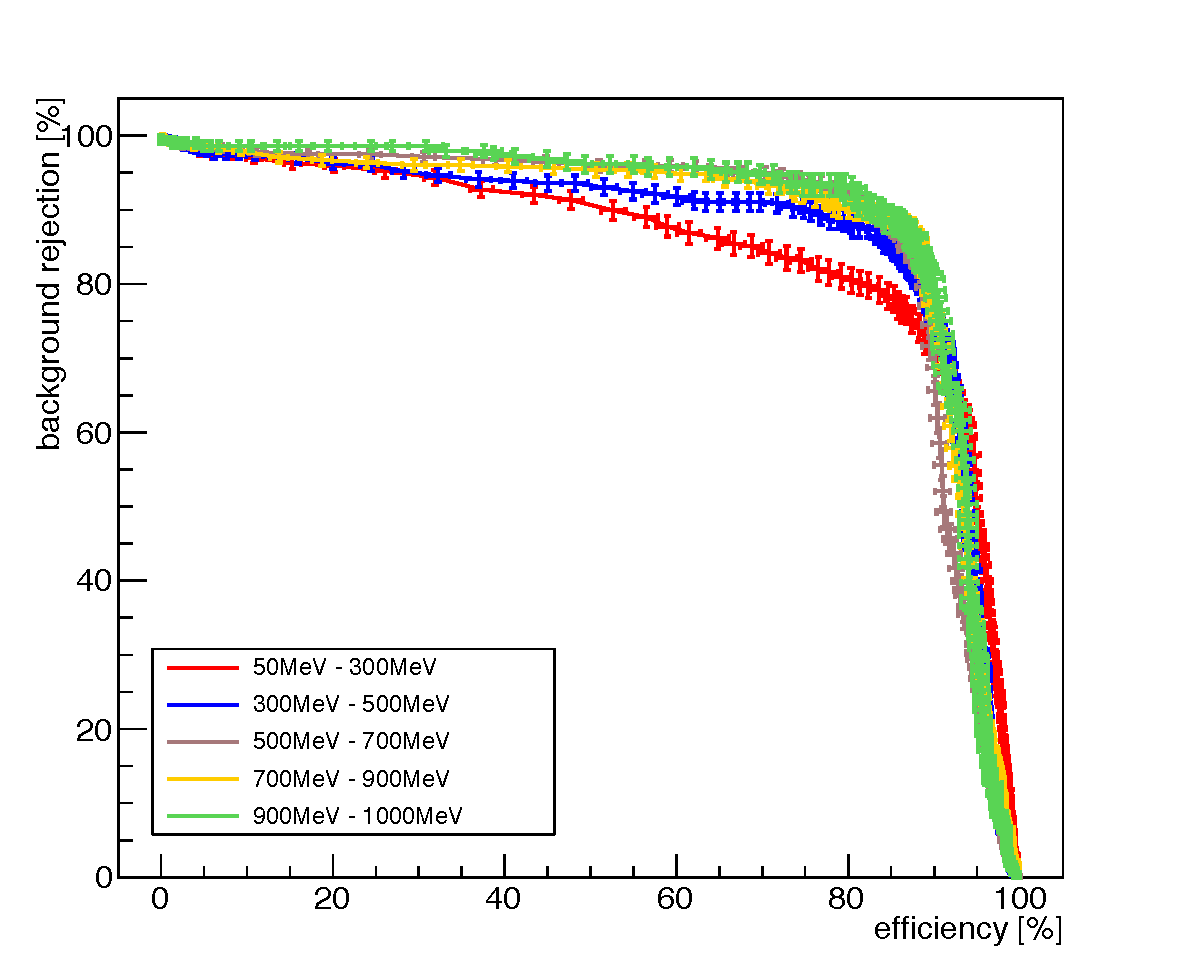
\includegraphics[width=0.8\textwidth]{annex_eff-bgdrej-diffen.pdf}
\end{cdrfigure}


\subsection{Neutrino Event Reconstruction and Classification}

In Qscan, a multivariate analysis (MVA) was used to separate particle types based on the spatial characteristics of their clusters
\cite{WA105_TDR,LAGUNA-LBNO-deliv,Stahl:2012exa}.
First step performs a principal components analysis (PCA), transforming the axes to lie along the 
cluster direction and perpendicular to it. Several quantities are then calculated to 
characterize the cluster: the lateral spread, the mean charge-weighted inverse distance of hits to the primary cluster axis
(this is expected to distinguish effectively between showers and tracks), the $dE/dx$.
These variables are then fed into Boosted Decision Trees analyses, 
each calculating the signal and background likelihoods for a particular particle hypothesis.
Currently muon, electron, proton and charged pion hypotheses are considered. It is anticipated that these likelihoods will be used in various ways by downstream analysis code, depending on the needs of the specific analysis.
In the present analysis, the BDT results for muon and electron hypotheses are used to identify lepton clusters and classify events. The signal and background distributions for these hypotheses are shown in 
Figure~\ref{fig:recoannexeventclassification}.

The overall performance of the reconstruction chain (from clustering to PID) has been estimated with a simple binned lepton flavor analysis, 
to understand its ability to distinguish $\nu_{e}$ and $\nu_{\mu}$ events.
If a single lepton flavor is identified in the event, then the event is considered as a signal event of the observed lepton flavor. 
If neither or both lepton flavors are identified, the event is discarded.
Numbers of events correctly reconstructed is above 90$\%$ for $\nu_{\mu}$-CCQE events.

%\fixme{Refer to the LAGUNA-LBNO PID plots}


\begin{cdrfigure}[LAGNUA-LBNO event classification]{recoannexeventclassification}
{Plots showing signal and background distributions for electron (a) and muon (b) MVA hypotheses. 
Background consists of all particles not corresponding to the relevant signal type.}
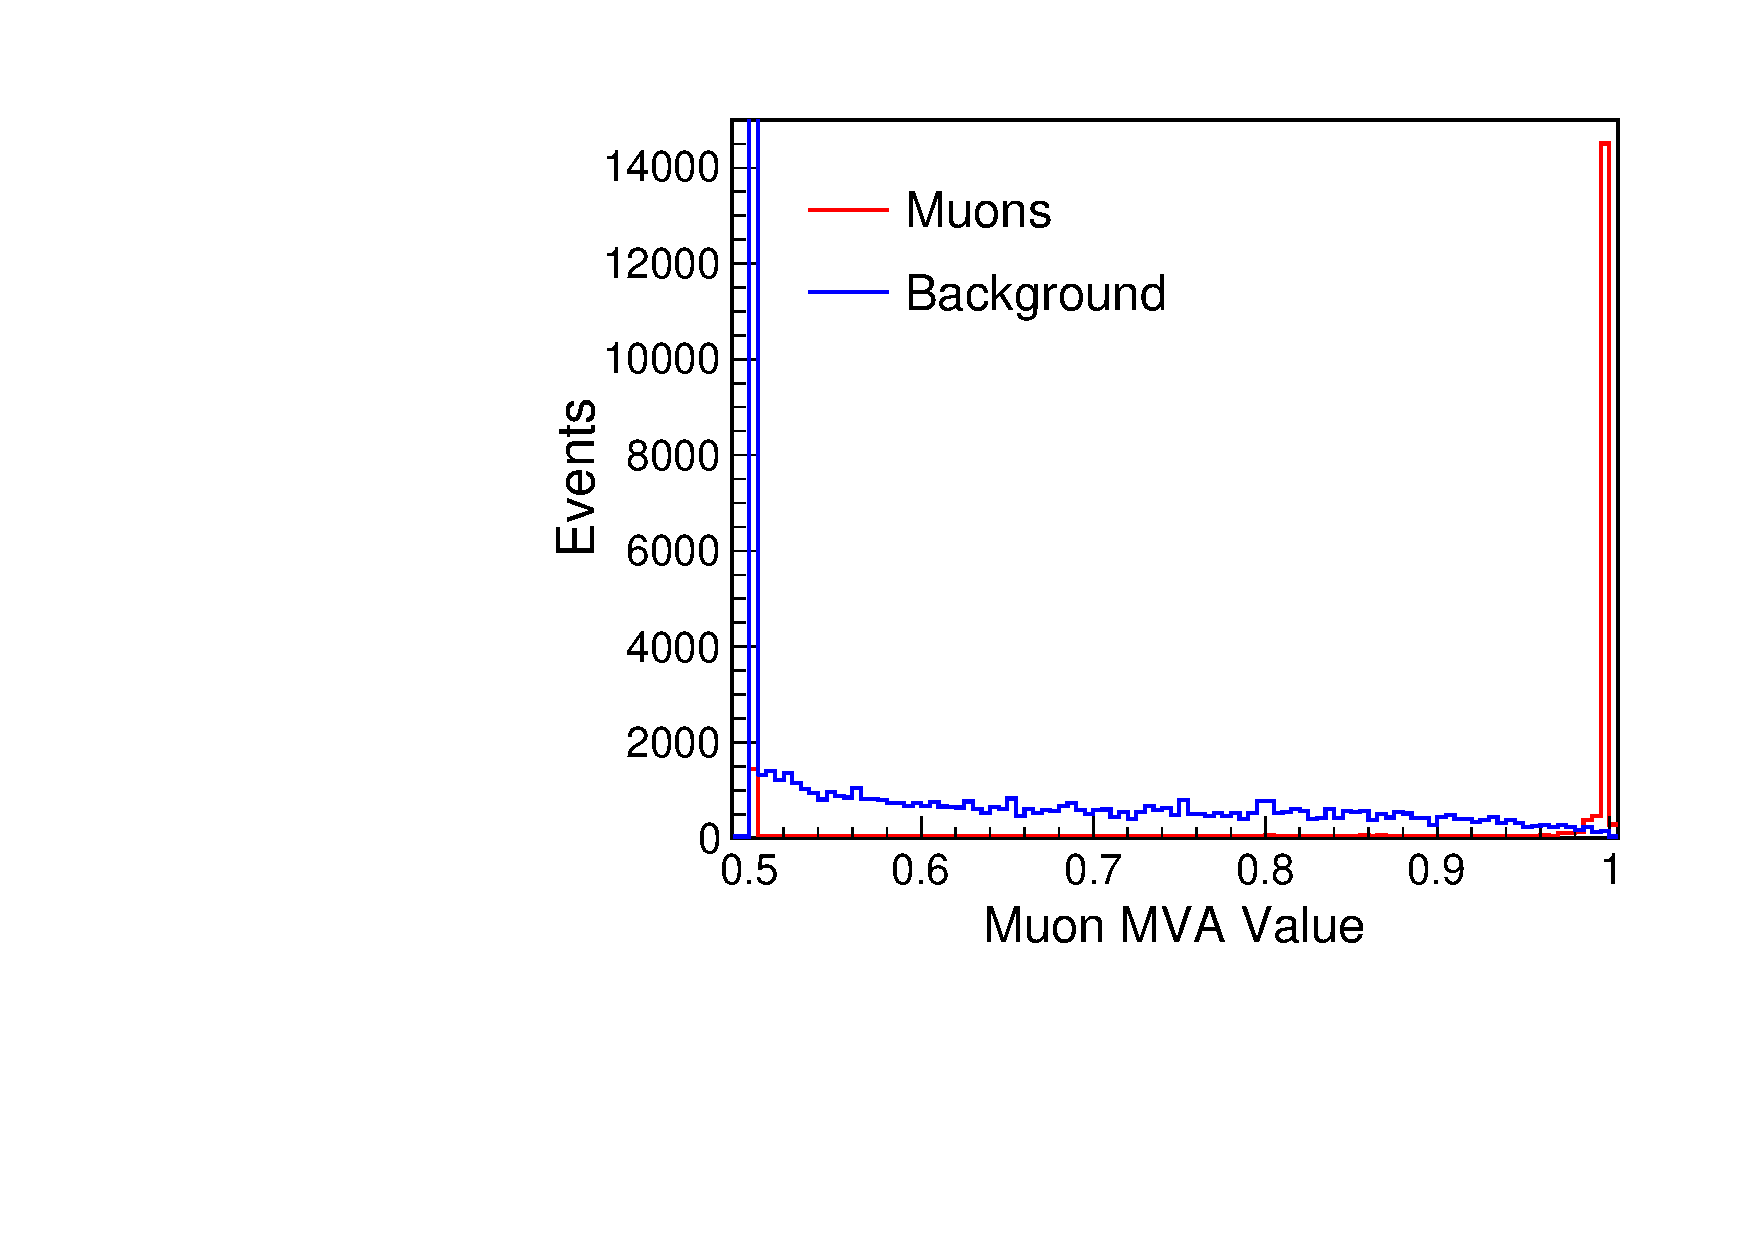
\includegraphics[width=0.49\textwidth]{laguna_lbno_pid_muons.pdf}
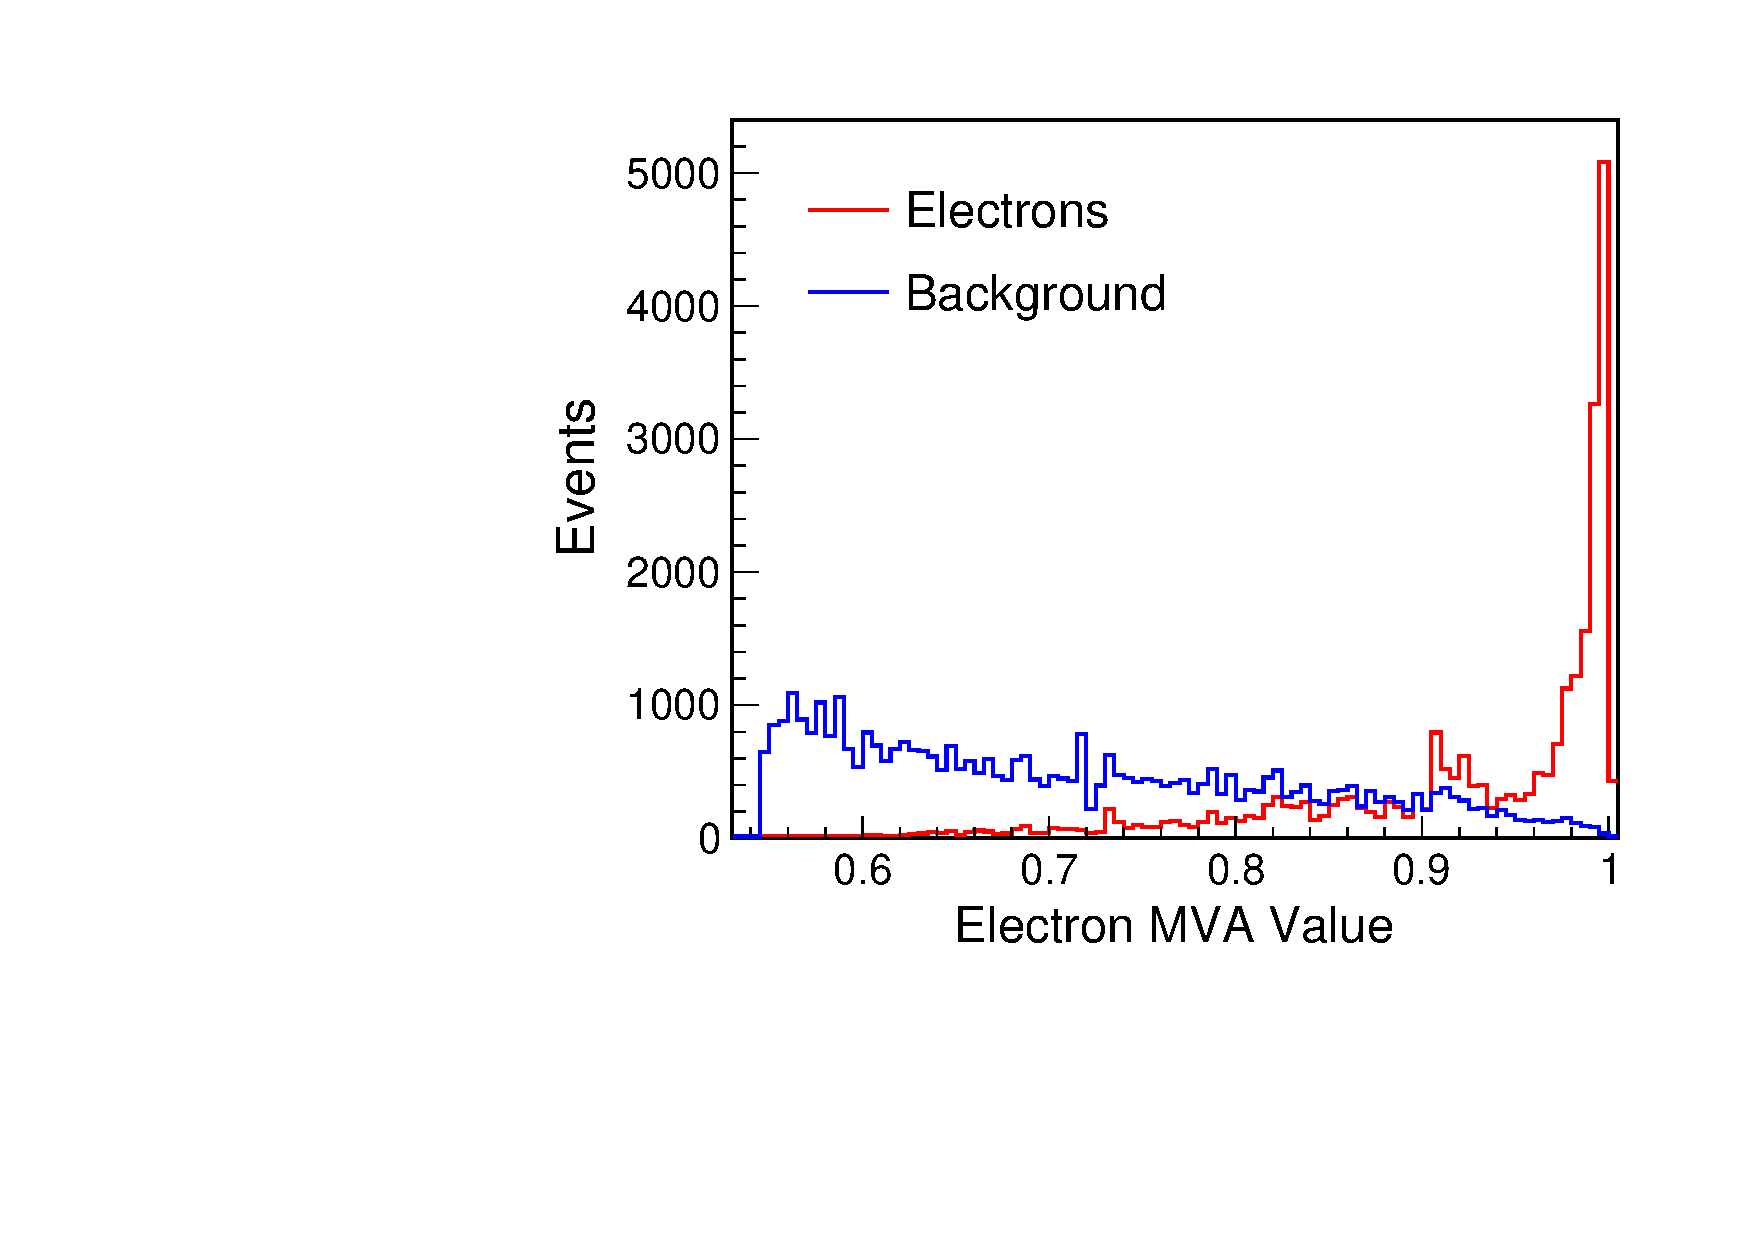
\includegraphics[width=0.49\textwidth]{laguna_lbno_pid_electrons.pdf}
\end{cdrfigure}

%\fixme{Talk about energy reconstruction here:}

For accepted events, the neutrino energy is estimated  assuming a CCQE event and using the two-body approximation, and also calorimetrically.
The calorimetric reconstruction takes account of the quenching factors for the different particles by 
assuming that all hits not associated with the lepton cluster are due to hadronic activity.
Figure~\ref{fig:recoannexrecoenergynue} shows the results of the kinematic energy reconstruction for CCQE events, and  Figure~\ref{fig:recoannexrecoenergynumu} the results of the calorimetric energy reconstruction.
It is seen that for high-energy muons, the measured energy saturates. This is due to the muon escaping the detector volume. 


%\fixme{Refer to the LAGUNA-LBNO Energy plots}


\begin{cdrfigure}[LAGNUA-LBNO electron neutrino energy measurement]{recoannexrecoenergynue}
{Dual-phase LArTPC neutrino energy measurement. Distributions of reconstructed neutrino energy versus true neutrino energy, assuming two-body kinematics. 
Plots shown are for $\nu_{e}$ CCQE (a) and $\nu_{\mu}$ CCQE (b).}
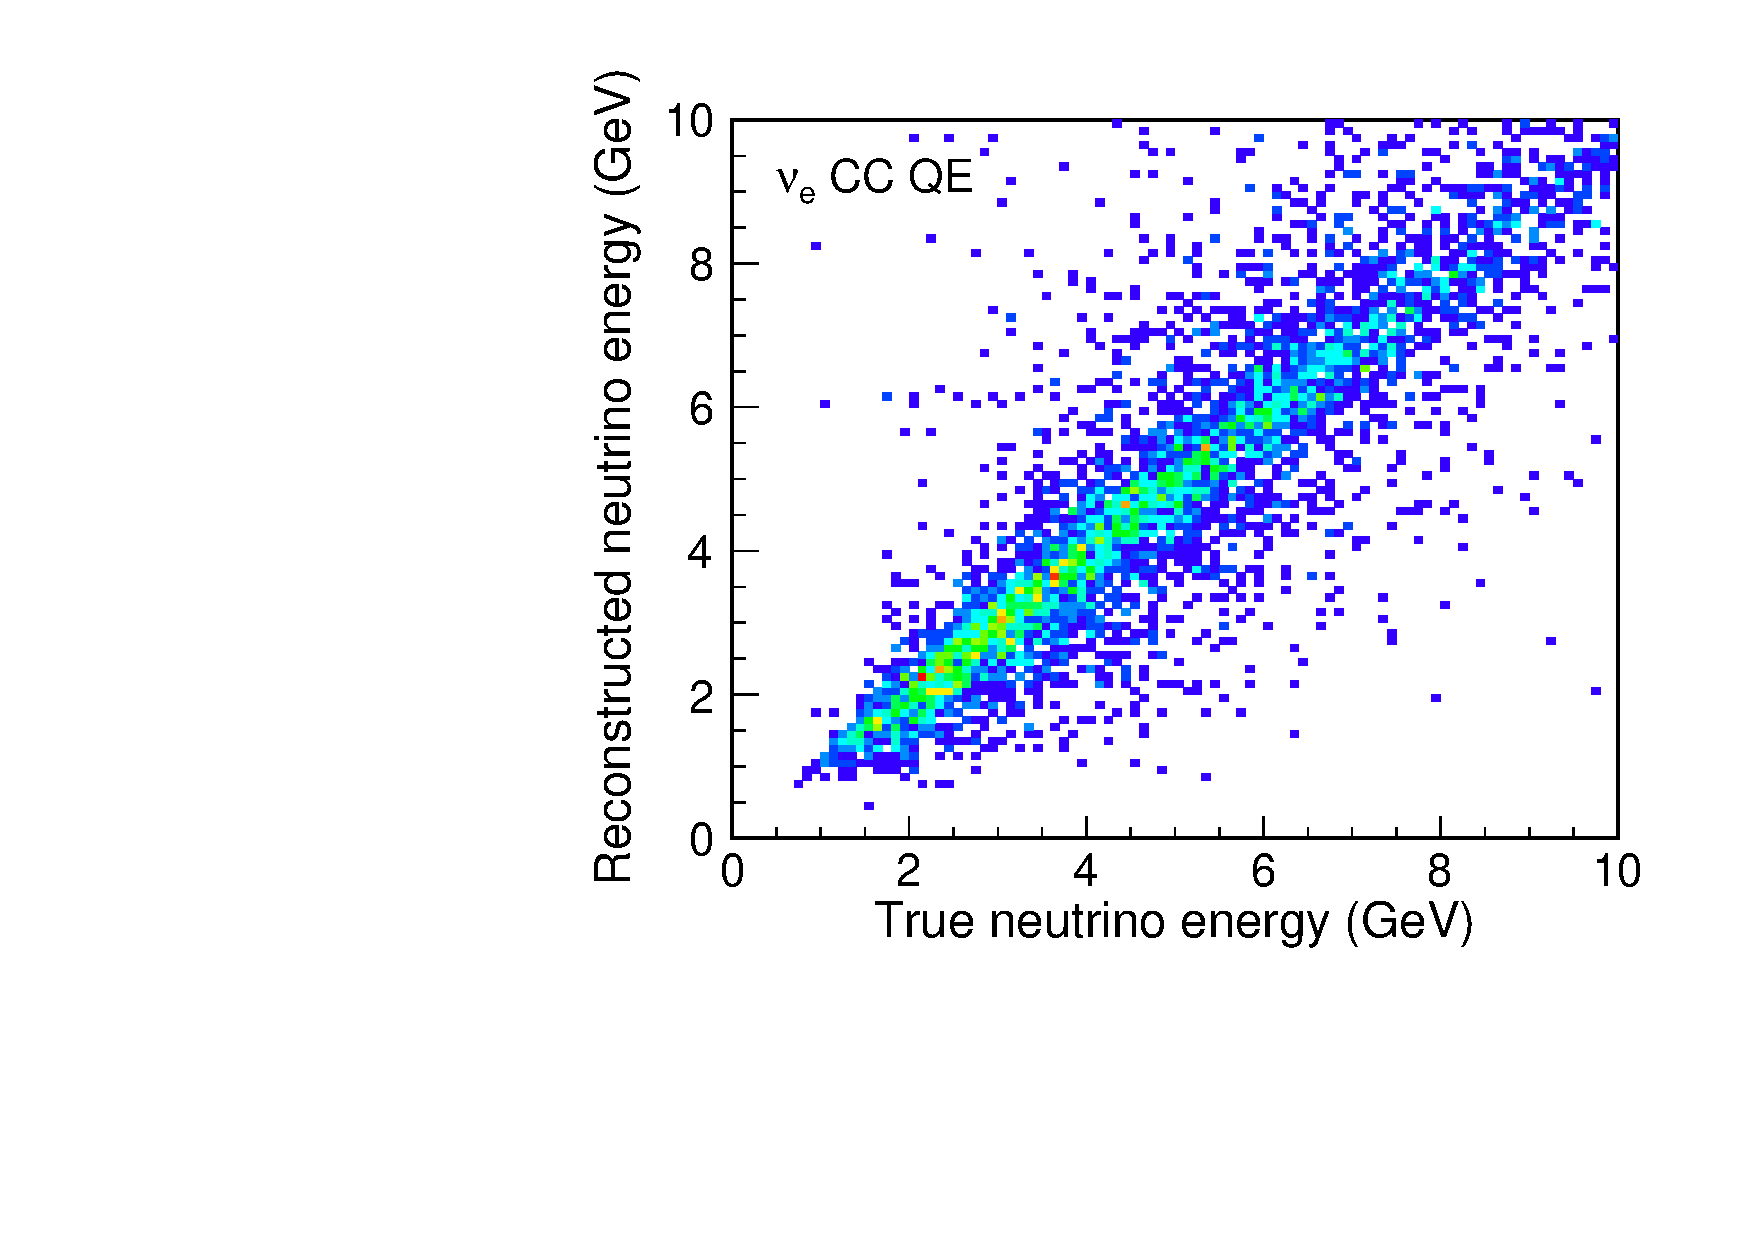
\includegraphics[width=0.49\textwidth]{laguna_lbno_recoenergy_nue_ccqe_annex.pdf}
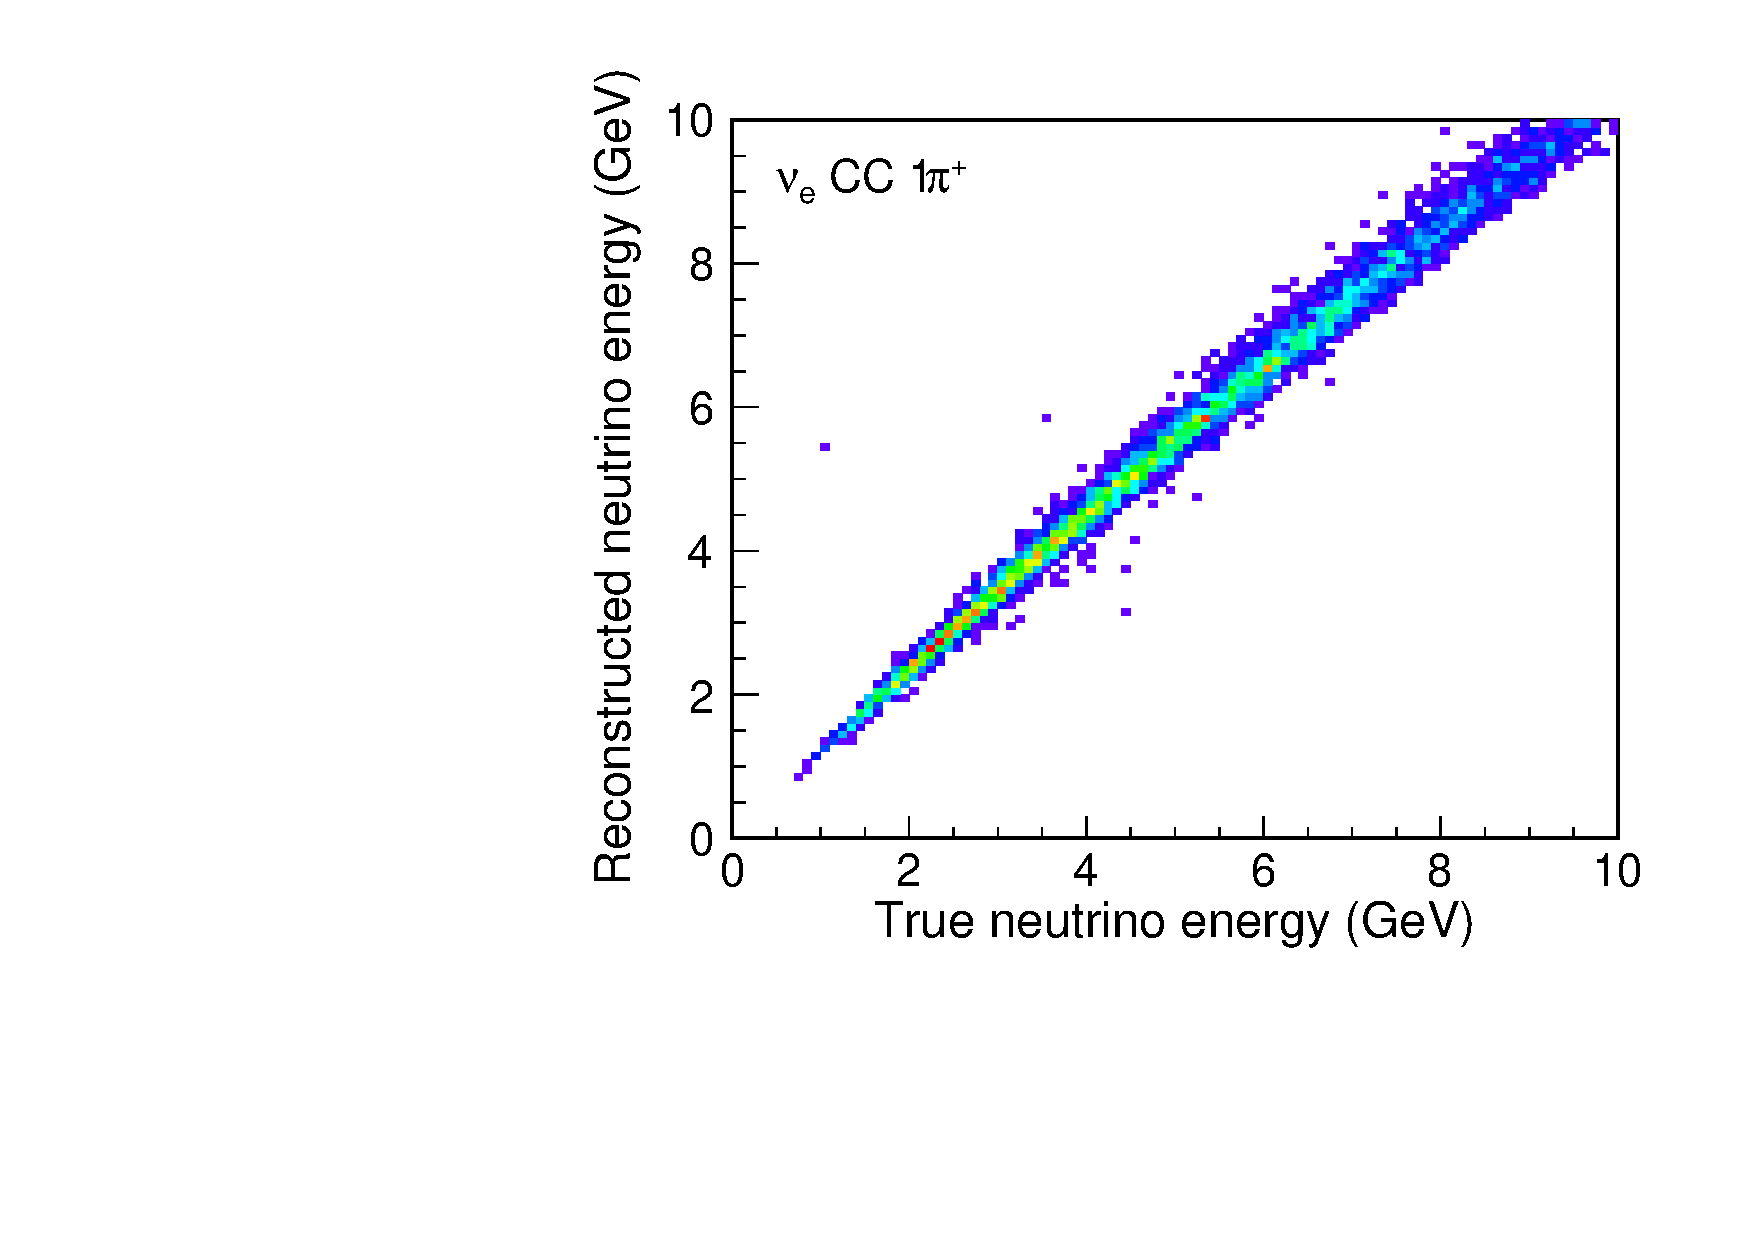
\includegraphics[width=0.49\textwidth]{laguna_lbno_recoenergy_nue_ccres_annex.pdf}
\end{cdrfigure}

\begin{cdrfigure}[LAGNUA-LBNO muon neutrino energy measurement]{recoannexrecoenergynumu}
{Dual-phase LArTPC neutrino energy measurement. Distributions of reconstructed neutrino energy versus true neutrino energy, using calorimetric energy estimation. 
Plots shown are for  $\nu_{e}$  CC1$\pi^{+}$ (a) and $\nu_{\mu}$  CC1$\pi^{+}$ (b).}
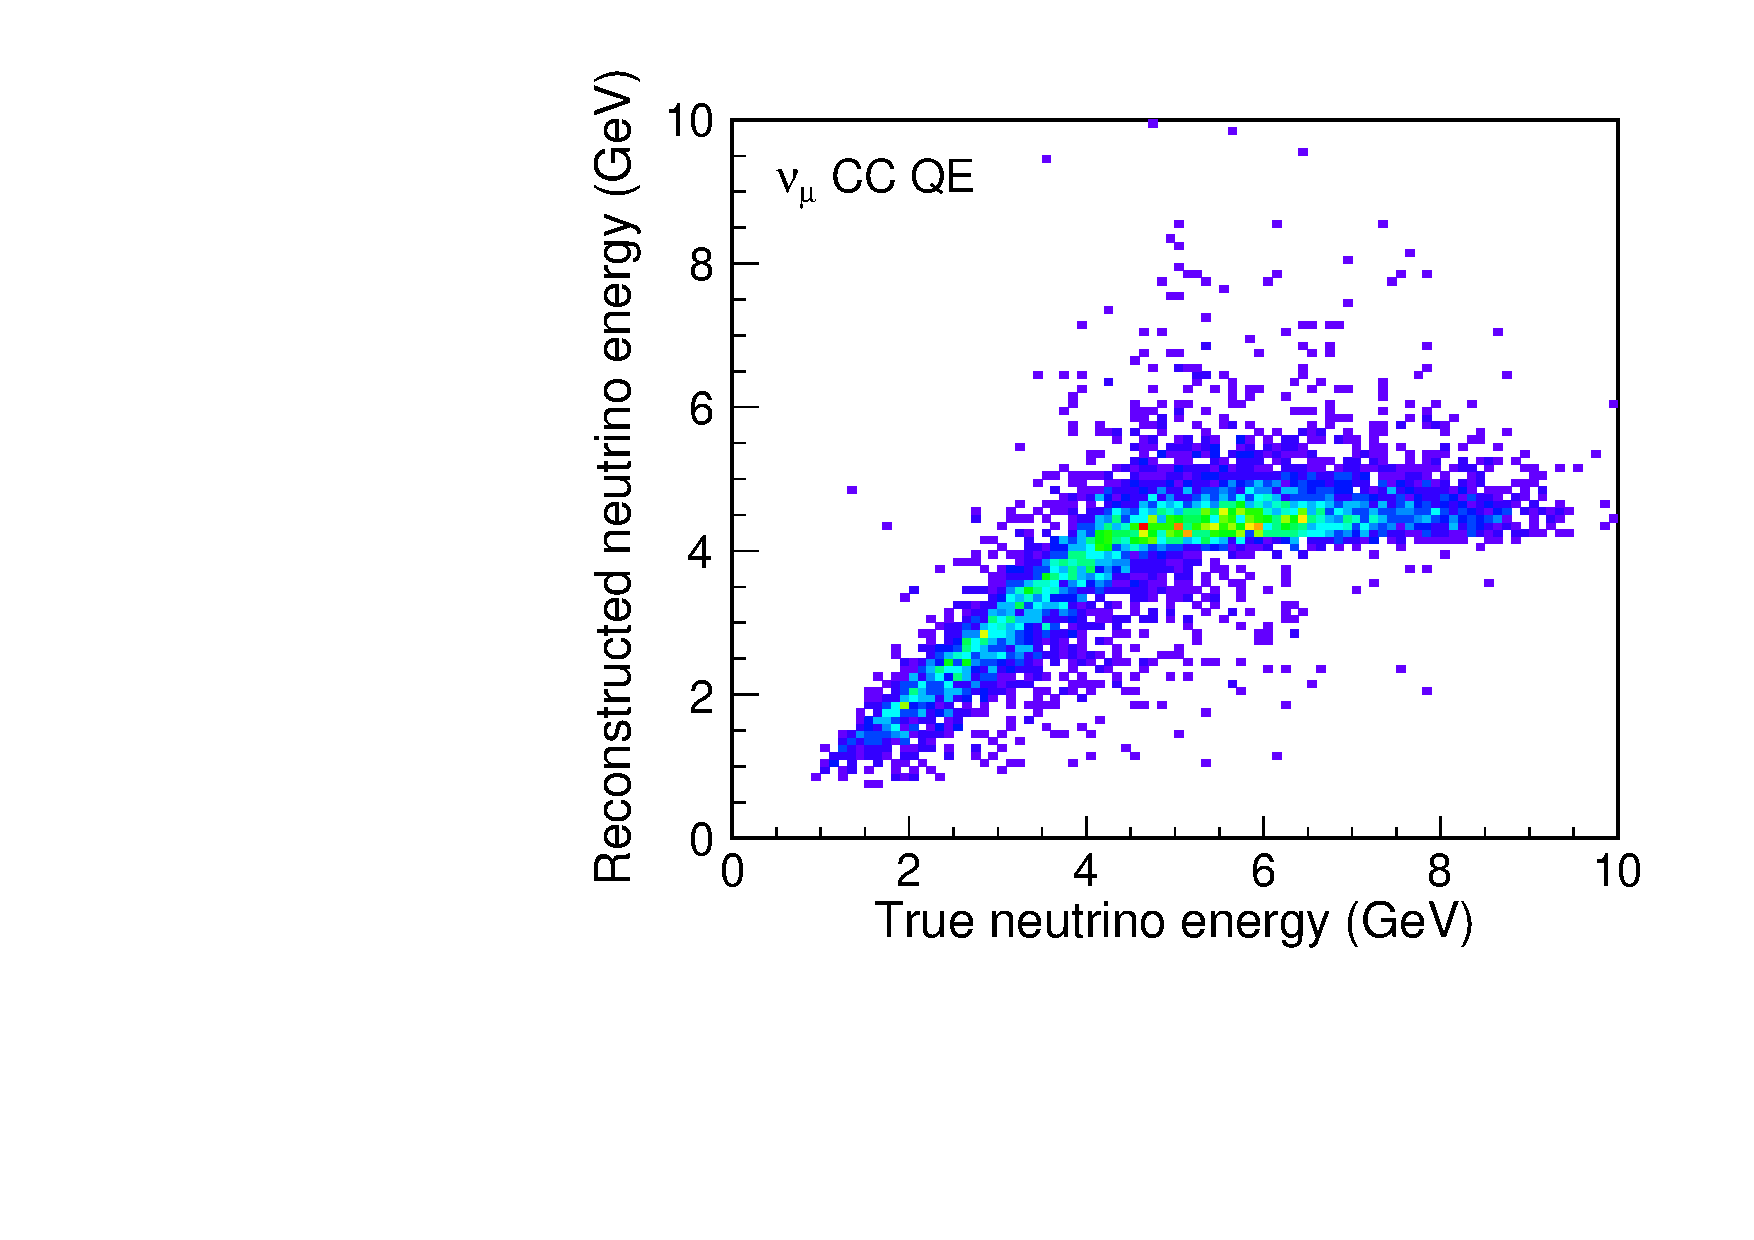
\includegraphics[width=0.49\textwidth]{laguna_lbno_recoenergy_numu_ccqe_annex.pdf}
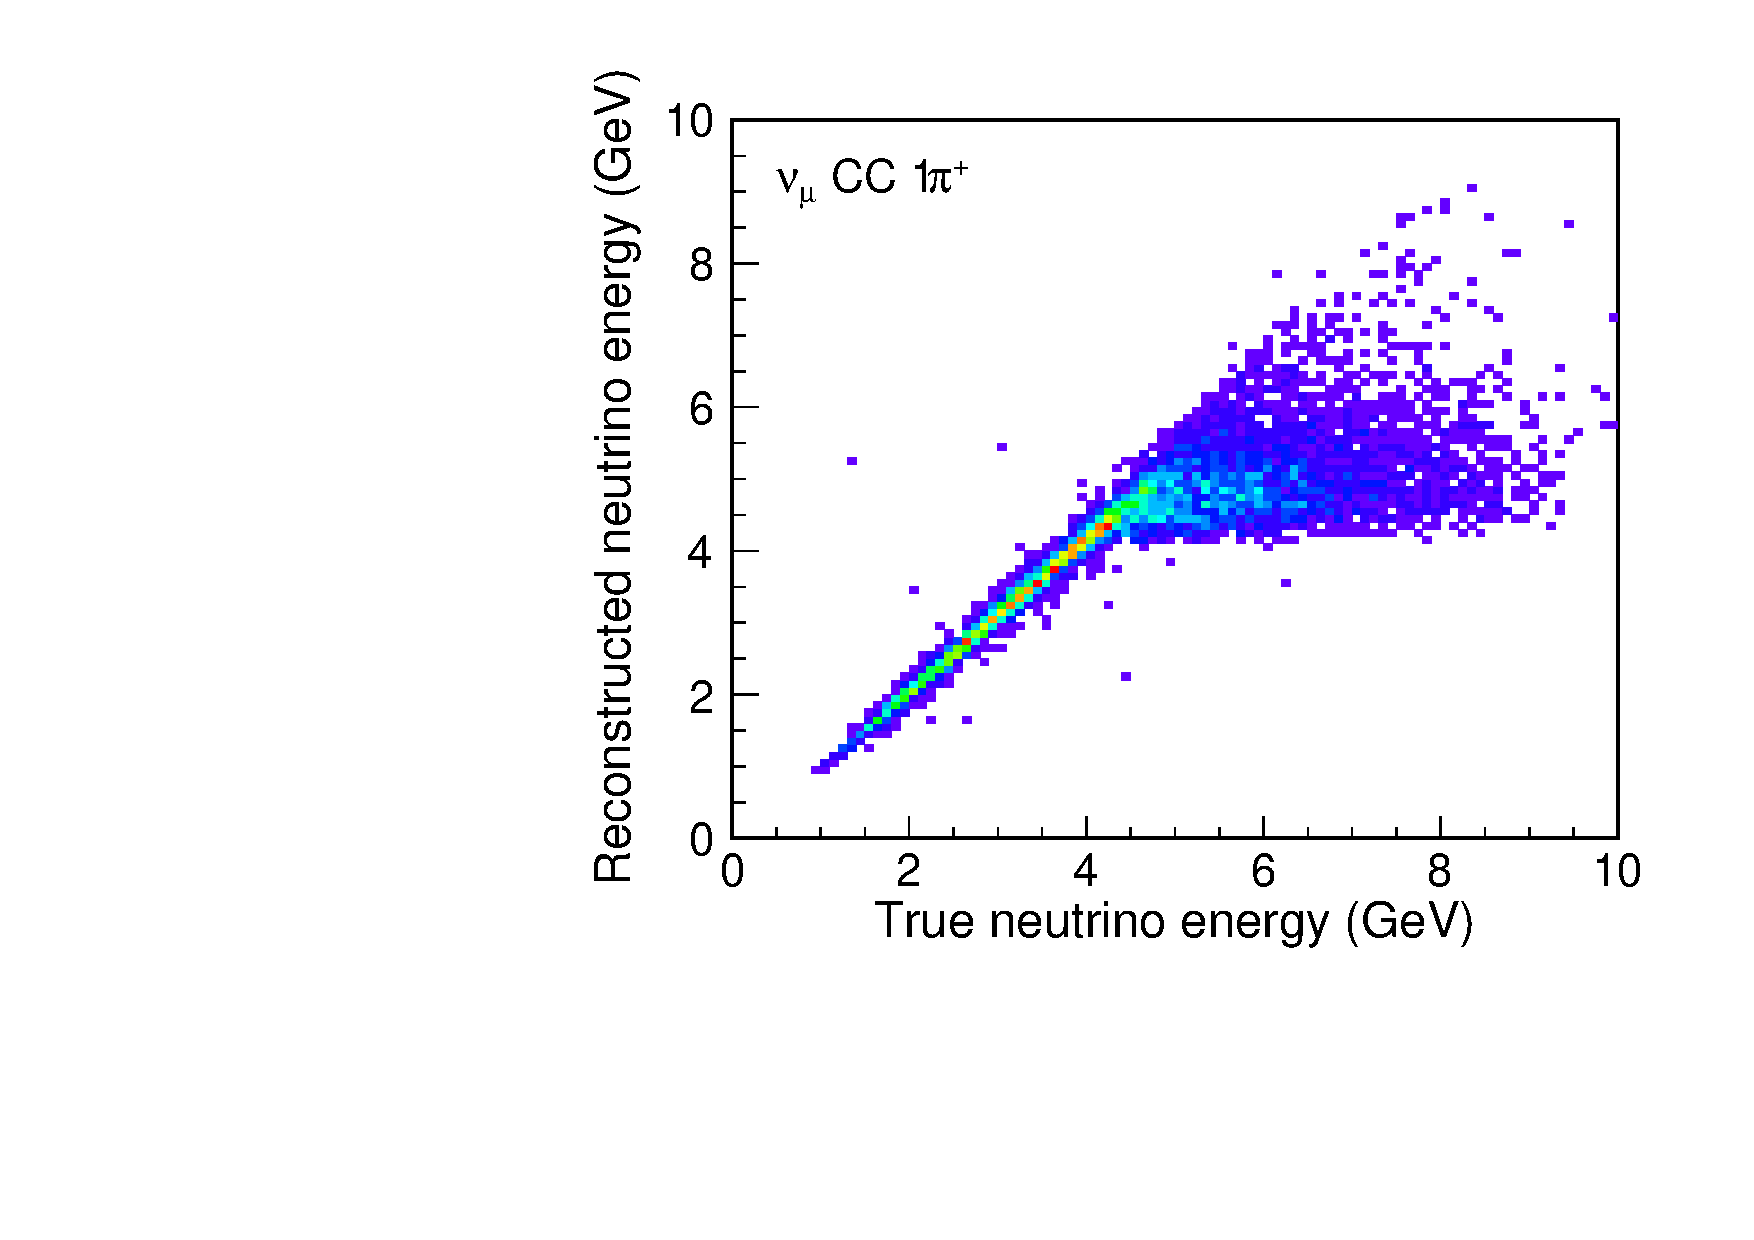
\includegraphics[width=0.49\textwidth]{laguna_lbno_recoenergy_numu_ccres_annex.pdf}
\end{cdrfigure}

%\fixme{Be sure to properly reference LAGUNA-LBNO design study: }
%\cite{WA105_TDR}
%\cite{LAGUNA-LBNO-deliv}
%\cite{LAGUNA-LBNO-EOI}


\subsection{Calibration}

In order to meet the requirements of high detection efficiency, efficient and
pure particle identification, excellent energy resolution, and small systematic
uncertainties on these performance parameters, calibrations of the detector
will be needed.  {\it In situ} calibration techniques using data collected by the FD
under identical conditions as used for physics analyses are the most desirable.
These include studying cosmic-ray events and non-fiducial interactions.  But not
all performance measures can be calibrated in this way.  A laser calibration system
will constrain the detector alignment as well as measure any residual space-charge effects
(which are expected to be very small underground) and other sources of field non-uniformity,
as well as provide timing calibration and crosscheck the response to drifting charge.  
The electronics will be outfitted with
charge-injection calibration systems so that non-uniformities in the electronics response
can be corrected in a time-dependent fashion.  The response to charged particles of known
energy and particle type will rely on test-beam data from LArIAT and the CERN test
experiments \cernsingleproto{} and \cerndualproto.
